%% Documentclass:
\documentclass[OpenMind]{stjour}

%% Or,

%% Manuscript, for double spaced, larger fonts
% \documentclass[manuscript]{stjour}
%% Only needed if you use `manuscript' option
% \journalname{Open Mind}

%%%%%%%%%%%%%%%%%%%%%%%%%%%%%%%%%%%%%%%%%%%%%%%%%%
%% For production only, not authors:
%%\documentclass[OpenMind,finalfonts]{stjour}

%%%%%%%%%%% Please supply information %%%%%%%%%%%%%%%%%%%%%%%%%

%% For Open Mind:
%% Supplementary Materials:
\supplementslinks{dx.doi.org/10.1098/rsif.2013.0969}

%% If no conflicts, this command doesn't need to be used
%% \conflictsofinterest{}

%%%%%%%%%%% to be supplied by MIT Press, only %%%%%%%%%%%%%%%%%

\citation{Niyogi, R. K., Breton, Y.-A., Solomon,
R. B., Conover, K.,\\ Shizgal, P., Dayan, P. (2015).\\ 
Optimal indolence: a normative microscopic approach to work and leisure. Open Mind 1(1):
1−12.}

\received{20 October 2013}
\accepted{7 November 2013}
\published{26 January 2014}

%% DOI address:
\setdoi{10.1098/rsif.2013.0969}

%%%%%%%% End MIT Press commands %%%%%%%%%%

%%%%%%%%%%%%%%%%%%%%%%%%%%%%%%%%%%%%%%%%%%%%%%%%%%%%%%%%%%%%%%%
%% author definitions should be placed here:

%% example definition
\def\taupav{\tau_{\mathrm{Pav}}}

\usepackage{csquotes}
\usepackage{tabularx}
\usepackage{threeparttable}
\usepackage{booktabs}


\begin{document}

\title{Polite speech emerges from competing social goals}
%\subtitle{Modeling polite speech} %% Optional subtitle

%% If shortened title for running head is needed so that the article title can fit
%%   in the running head, use [] argument, ie,
%%
%%   \title[Shortened Title for Running Head]{Title of Article}
%%   \subtitle{Subtitle Here}

%%% Author/Affil
%% Since we use \affil{} in the argument of the \author command, we
%% need to supply another version of the author names, without \affil{}
%% to be used for running heads:

\author[Yoon, Tessler, Goodman, \and Frank]
{Erica J. Yoon\affil{1, +�},
Michael Henry Tessler\affil{2, +�}, Noah D. Goodman\affil{1},\\
\and Michael C. Frank\affil{1}}

\affiliation{1}{Department of Psychology, Stanford University}
\affiliation{2}{Department of Brain and Cognitive Sciences, MIT}
%\affiliation{*}{Corresponding author}
\affiliation{+}{These authors contributed equally to this work. }


%ie.
%\affiliation{1}{Gatsby Computational Neuroscience Unit, University
%College London, London, United Kingdom} 

%ie
%\affiliation{2}{Center for Studies in
%Behavioral Neurobiology, Concordia University, Montreal, Quebec,
%Canada}

\correspondingauthor{Erica J. Yoon}{ejyoon@stanford.edu}

% ie,
%\correspondingauthor{Ritwik K. Niyogi}{ritwik.niyogi@gatsby.ucl.ac.uk}

\keywords{politeness, computational modeling, communicative goals, pragmatics}

%ie
%\keywords{work, leisure, normative, microscopic,  reinforcement learning, economics}

\begin{abstract}
Language is a remarkably efficient tool for transmitting information.
Yet human speakers make statements that are inefficient, imprecise, or
even contrary to their own beliefs, all in the service of being polite.
What rational machinery underlies polite language use? Here, we show
that polite speech emerges from the competition of three communicative
goals: to convey information, to be kind, and to present oneself in a
good light. We formalize this goal tradeoff using a probabilistic model
of utterance production, which predicts human utterance choices in
socially-sensitive situations with high quantitative accuracy, and we
show that our full model is superior to its variants with subsets of the
three goals. This utility-theoretic approach to speech acts takes a step
towards explaining the richness and subtlety of social language use.
\end{abstract}



\section{Introduction}\label{introduction}

We don't always say what's on our minds. Although \enquote{close the
window!} could be sufficient, we dawdle, adding \enquote{can you
please\ldots{}?} or \enquote{would you mind\ldots{}?} Rather than tell
an uncomfortable truth, socially-aware speakers exaggerate
(\enquote{Your dress looks great!}) and prevaricate (\enquote{Your poem
was so appropriate to the occasion}). Such language use is puzzling for
classical views of language as information transfer \citep{buhler1934, frank2012, jakobson1960, shannon1948}. On the classical view,
transfer ought to be efficient and accurate: Speakers are expected to
choose succinct utterances to convey their beliefs \citep{grice1975, searle1975}, and the information conveyed is ideally truthful to the extent of
a speaker's knowledge. Polite speech violates these basic expectations
about the nature of communication: It is typically inefficient and
underinformative, and sometimes even outright false. Yet even young
speakers spontaneously produce requests in polite forms \citep{axia1985}, 
and adults use politeness strategies pervasively -- even while
arguing \citep{holtgraves1997}, and even though polite utterances may risk
high-stakes misunderstandings \citep{bonnefon2011risk}.

If politeness only gets in the way of effective information transfer,
why be polite? Most obvious is the fact that we have social
relationships to maintain, and most linguistic theories assume speaker
behavior is motivated by these concerns, couched as either polite maxims
\citep{leech1983}, social norms \citep{ide1989}, or aspects of a speaker and/or
listener's identity, known as \emph{face} \citep{brown1987, goffman1967}. 
Face-based theories predict that when a speaker's
intended meaning contains a threat to the listener's face or self-image
(and potentially the speaker's face), her messages will be less direct,
less efficient, and possibly untruthful. Indeed, when interpreting
utterances in face-threatening situations, listeners readily assume that
speakers intend to be polite \citep{bonnefon2009}.
How this socially-aware calculation unfolds, however, is not well
understood. Adopting an example from \citet{bonnefon2009}, when should
a speaker decide to say something false (\enquote{Your poem was great!}
said of an actually-mediocre poem) rather than to tell the truth
(\enquote{Your poem was bad}) or to be indirect (\enquote{Some of the
metaphors were tricky to understand.})? How do the speaker's goals enter
into the calculation?

We propose a utility-theoretic solution to the problem of understanding
polite language, in which speakers choose their utterance by attempting
to maximize utilities that represent competing communicative goals.
Under the classic pragmatic view of language production, speakers want
to be informative and convey accurate information as efficiently as
possible \citep{goodman2016, grice1975}; this desire for
informative and efficient communication we call \emph{informational
utility}. In addition, speakers may want to be kind and make the
listener feel good (i.e., save the listener's face), for example, by
stating positive remarks about the listener. The utility that underlies
this goal is a \emph{prosocial utility}.

If a speaker wants to be informative and kind, then she would ideally
produce utterances that satisfy both goals. The nuances of reality,
however, can make it difficult to satisfy both goals. In particular,
when the true state of the world is of low value to the listener (e.g.,
the listener's poem was terrible), informational and prosocial goals
pull in opposite directions. Informational utility could be maximized by
stating the blunt truth (\enquote{your poem was terrible.}) but that
would very likely hurt the listener's feelings and threaten the
listener's self-image (low prosocial utility); prosocial utility could
be maximized through a white lie (\enquote{your poem was amazing}), but
at the cost of being misleading (low informational utility). In such
situations, it seems impossible to be both truthful and kind. A first
contribution of our work here is to formalize the details of this
tradeoff in order to predict experimental data.

A second contribution of our work is to develop and test a new
theoretical proposal. We propose that speakers may navigate their way
out of the truth-kindness conflict by signaling to the listener that
they care about both of the goals, even while they are genuinely unable
to fulfill them. We formalize this notion of \emph{self-presentational
utility} and show that it leads speakers to prefer indirect speech:
utterances that provide less information relative to alternatives with a
similar meaning.

We look at indirect speech in this paper through negated adjectival
phrases (e.g., \enquote{It \emph{wasn't bad}}). The relationship between
negation and politeness is a topic of long-standing interest to
linguists and psychologists \citep{stoffel1901intensives, stern1931meaning, bolinger1972degree, horn1989natural}. 
Comprehending negation, as a logical operation, can be
psychologically more complex than comprehending an unnegated assertion,
resulting in difficulty in processing of negations \citep[\citealp{clark1972}; see][for an underlying pragmatic
explanation]{nordmeyer2014} as well as failure to recognize or recall the asserted
content \citep{lea2002, macdonald1989}. Our interest
in negation, however, is for its information-theoretic properties:
Negating an assertion that has a specific meaning results in a meaning
that is less precise and lower in informativity (e.g., negating
\enquote{Alex has blue eyes} results in the statement that \enquote{Alex
has eyes that are some color other than blue}). In our paradigm, we use
negation as a way of turning a relatively direct statement (\enquote{It
was terrible}) into an indirect statement (\enquote{It wasn't terrible})
whose interpretation includes some possibilities that are consistent
with or close to the unnegated statement (i.e., the poem was not
terrible, but it was still pretty bad).

Multifactorial, verbal theories -- like previous proposals regarding
politeness -- are very difficult to relate directly to behavioral data.
Therefore, to test our hypotheses about the factors underlying the
production of polite language (what we refer to as its utility
structure), we take a model comparison approach. We do this by
formalizing the trade-off between different combinations of speakers'
utilities in a class of probabilistic models of language use \citep[the
Rational Speech Act (RSA) framework;][]{frank2012, goodman2016}, 
with a particular focus on models with and without the
self-presentational utility. In this framework, speakers are modeled as
agents who choose utterances by reasoning about their potential effects
on a listener, while listeners infer the meaning of an utterance by
reasoning about speakers and what goals could have led them to produce
their utterances. These models build on the idea that human social
cognition can be approximated via reasoning about others as rational
agents who act to maximize their subjective utility \citep{baker2009action}, 
a hypothesis which has found support in a wide variety
of work with both adults and children \citep[e.g.,][]{jara2016naive, liu2017ten}.
Indeed, this class of pragmatic language models has been productively
applied to understand a wide variety of complex linguistic behaviors,
including vagueness \citep{lassiter2017adjectival}, hyperbole \citep{kao2014}, 
and irony \citep{kao2015}, among
others.

\begin{figure}[!h]
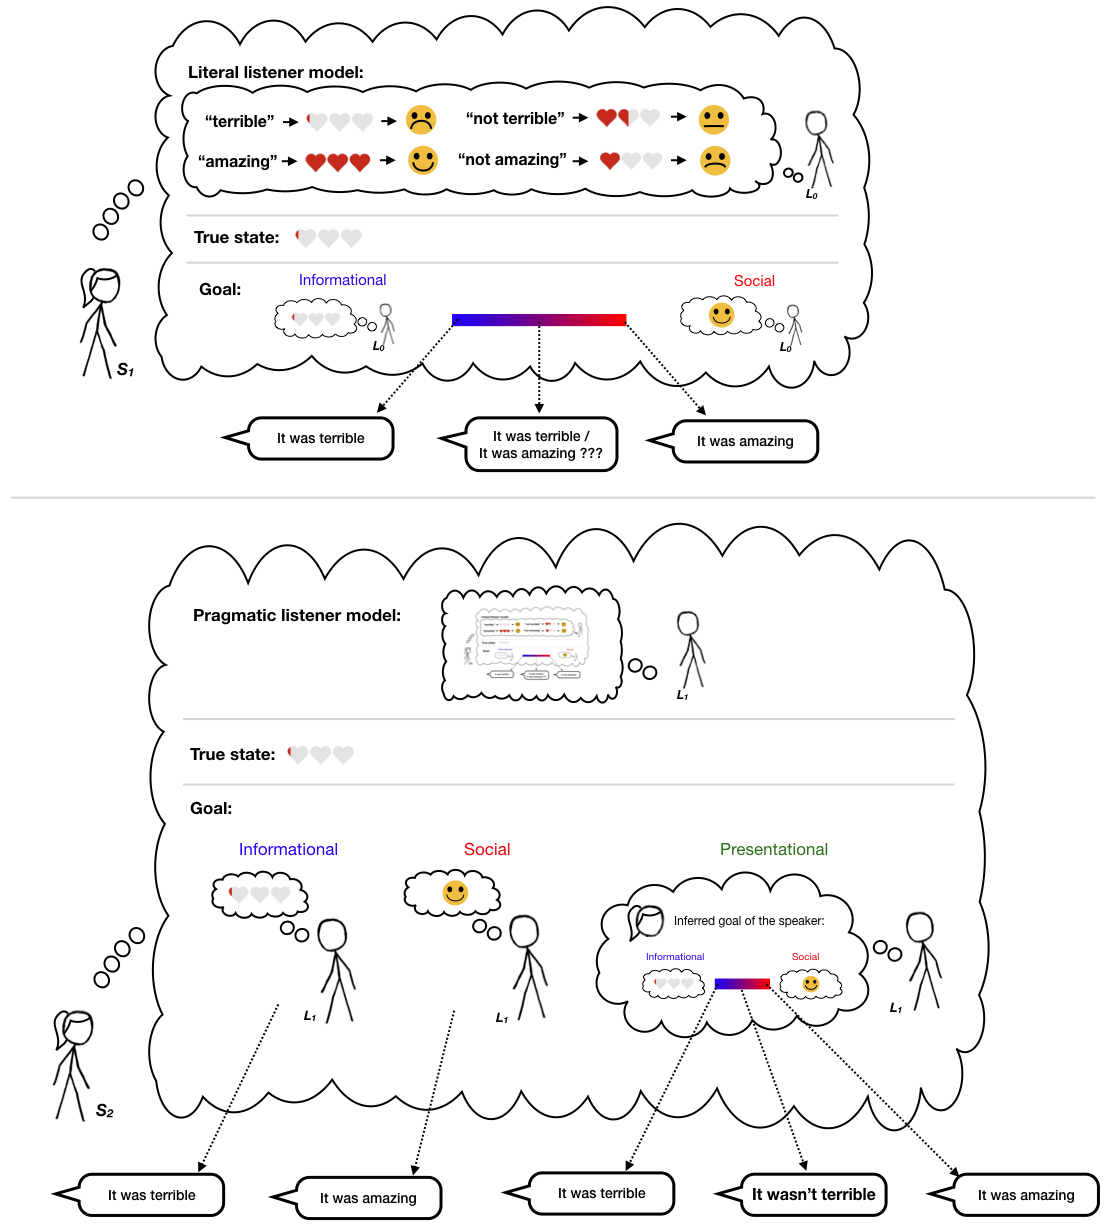
\includegraphics[width=\linewidth]{fig/model} \caption{Diagram of the model, showing $S_1$ (a first-order polite speaker) and $S_2$ (a higher-order polite speaker capable of self-presentational goals) Top: First-order polite speaker ($S_1$) produces an utterance by thinking about: (1) the true state of the world (i.e., how good a given performance was); (2) the reasoning of literal listener who updates his beliefs about the true state via the literal meanings of utterances (e.g., “not terrible” means approximately 1.5 heart out of 3 hearts) and their affective consequences for the listener; and (3) her goal of balancing informational and social utilities. Bottom: Second-order polite speaker ($S_2$) produces an utterance by thinking about (1) the true state; (2) the pragmatic listener $L_1$ who updates his beliefs about the true state and the first-order speaker $S_1$’s goal (via reasoning about the $S_1$ model); and (3) her goal of balancing informational, prosocial, and self-presentational utilities. Different utterances shown correspond to different weightings of the utility components.}\label{fig:model}
\end{figure}

\section{Model}\label{model}

RSA models are defined recursively such that speakers \(S\) reason about
listeners \(L\), and vice versa. We use a standard convention in
indexing and say a pragmatic listener \(L_1\) reasons about the intended
meaning and goals that would have led a speaker \(S_1\) to produce a
particular utterance. \(S_1\) reasons about a \emph{literal listener}
\(L_0\), who is modeled as attending only to the literal meanings of
words (rather than their pragmatic implications), and hence grounds the
recursion (Figure \ref{fig:model}, top). The target of our current work
is a model of a polite speaker \(S_2\) who reasons about what to say to
\(L_1\) by considering some combination of informational, social, and
self-presentational goals (Figure \ref{fig:model}, bottom).

We evaluate our model's ability to predict human speaker production
behavior in situations where polite language use is expected. Our
experimental context involves a speaker (\enquote{Ann}) responding to
the request of their listener (\enquote{Bob}) to evaluate the listener's
(Bob's) creative product. For instance, Bob recited a poem and asked Ann
how good it was. Ann (\(S_2\)) produces an utterance \(w\) based on the
true state of the world \(s\) (i.e., the rating, in her mind, truly
deserved by Bob's poem) and a set of goal weights
\(\boldsymbol{\omega}\), that determines how much Ann prioritizes each
of the three possible goals, as well as a goal weight to project to the
listener (\(\phi\); more details below). Following standard practice in
RSA models, Ann's production decision is softmax, which interpolates
between choosing the maximum-utility utterance and probability matching \citep[via speaker optimality parameter \(\alpha\); ][]{goodman2013}:

\begin{equation}
P_{S_2}(w | s, \boldsymbol{\omega}) \propto \exp[\alpha \cdot U_{total}(w; s; \boldsymbol{\omega}; \phi) ] \label{eq:S2}
\end{equation}

We posit that a speaker's utility contains distinct components that
represent three possible goals that speakers may entertain:
informational, prosocial, and presentational. These components were
determined based on multiple iterations of preliminary experiments,
after which we conducted the preregistered test of our specified model
with the specific utilities that we report below \citep{yoon2016, yoon2017}.

We take the total utility \(U_{total}\) of an utterance to be the
weighted combination of the three utilities minus the utterance cost
\(C(w)\), which is used to capture the general pressure towards economy
in speech (e.g., longer utterances are more costly):

\begin{equation}
U_{total}(w; s; \boldsymbol{\omega}; \phi) = \omega_{inf} \cdot U_{inf}(w; s) + \omega_{soc} \cdot U_{soc}(w) + \omega_{pres} \cdot U_{pres}(w; \phi) - C(w). \label{eq:UTotal}
\end{equation}

First, a speaker may desire to be epistemically helpful, modeled as
standard \emph{informational utility} (\(U_{inf}\)). The informational
utility indexes the utterance's negative \emph{surprisal}, or amount of
information the listener (\(L_1\)) would still not know about the state
of the world \(s\) after hearing the speaker's utterance \(w\) (e.g.,
how likely is Bob to guess Ann's actual opinion of the poem):
\(U_{inf}(w) = \ln(P_{L_1}(s | w))\).

Speakers who optimize for informational utility produce accurate and
informative utterances while those who optimize for social utility
produce utterances that make the listener feel good. We define
\emph{social utility} (\(U_{soc}\)) to be the expected subjective
utility of the state \(V(s)\) implied to the pragmatic listener by the
utterance: \(U_{soc}(w) = \mathbb{E}_{P_{L_1}(s \mid w)}[V(s)]\). The
subjective utility function \(V(s)\) is a mapping from states of the
world to subjective values, which likely varies by culture and context;
we test our model when states are explicit ratings (e.g., numbers on a
4-point scale) and we assume the simplest positive linear relationship
between states \(s\) and values \(V(s)\), where the subjective value is
the numerical value of the state (i.e., the number of hearts). For
example, Bob would prefer to have written a poem deserving 4 points
(visualized as 3 hearts) rather than 1 point (visualized as 0 heart) and
the strength of that preference is 4-to-1.

Listeners who are aware that speakers can be both kind and honest could
try to infer the relative contribution of these two goals to the
speaker's behavior (e.g., by asking himself: \enquote{was Ann just being
nice?}). Thus, we use a pragmatic listener model who has uncertainty
about the speaker's goal weight (relative contribution of niceness
vs.~informativeness) in addition to their uncertainty about the state of
the world (number of hearts; Eq. \ref{eq:L1}). A speaker gains
presentational utility when her listener believes she has particular
goals, represented by a mixture parameter \(\phi\) weighting the goals
to be genuinely informative vs.~kind.

A sophisticated speaker can then produce utterances in order to appear
\emph{as if} she had certain goals in mind, for example making the
listener think that the speaker was being both kind and informative.
Such a \emph{self-presentational} goal may be the result of a speaker
trying to save their own face (\emph{I want the listener to see that I'm
a decent person}) and can result in different speaker behavior depending
on the intended, projected goal of the speaker (e.g., \emph{I want the
listener to think I'm being honest} vs. \emph{nice} vs.
\emph{both})\footnote{In principle, one could continue the recursion
  hierarchy and define a listener \(L_2\) who reasons about this clever
  speaker and tries to uncover the goals that the speaker was trying to
  convey to them; we think such reasoning is reserved for very special
  relationships and is unlikely to manifest in the more basic acts of
  polite language use that we study here.}.

The extent to which the speaker \emph{projects} a particular goal to the
listener (e.g., to be kind) is the utterance's \emph{presentational
utility} (\(U_{pres}\)). Formally,

\begin{equation}
U_{pres}(w; \phi) = \ln(P_{L_1}(\phi \mid w)) = \ln \int_s P_{L_1}(s, \phi \mid w).
\end{equation}

\noindent The speaker projects a particular weighting of informational
vs.~social goals (\(\phi\)) by considering the beliefs of listener
\(L_1\), who hears an utterance and jointly infers the speaker's
utilities and the true state of the world:

\begin{equation}
P_{L_1}(s, \phi | w) \propto P_{S_1}(w | s, \phi) \cdot P(s) \cdot P(\phi). \label{eq:L1}
\end{equation}

\noindent The presentational utility \(U_{pres}\) is the highest-order
term of the model, defined only for a speaker thinking about a listener
who evaluates a speaker (i.e., defined for the second-order speaker
\(S_2\), but not the first-order speaker \(S_1\)). Only the social and
informational utilities are defined for the first-order \(S_1\) speaker
(via reasoning about \(L_0\)); thus, \(S_1\)'s utility weightings can be
represented by a single number, the mixture parameter \(\phi\).
Definitions for \(S_1\) and \(L_0\) otherwise mirror those of \(S_2\)
and \(L_1\) and we use the same speaker optimality parameter for \(S_1\)
and \(S_2\) for simplicity; these sub-models are defined in the next
section and appear in more detail in the Supplementary Materials. The
complete model specification is in Fig. \ref{fig:bayesnet}.

Within our experimental domain, we assume there are four possible states
of the world corresponding identically to the value placed on a
particular referent (e.g., the 1-to-4 numeric rating of the poem the
speaker is commenting on), represented in terms of numbers of hearts
(Figure \ref{fig:model}): \(S = {s_0,...,s_3}\). In the experiment,
participants are told that the listener has no idea about the quality of
the product; thus, both listener models \(L_1\) and \(L_0\) assume
uniform priors P(s) over the four possible heart states. The pragmatic
listener's prior distribution over the first-order speaker's utility
weights \(P(\phi)\) encodes baseline assumptions about the relative
informativeness vs.~niceness listener's expect, which also plausibly
varies by culture and context; for simplicity, we assume this
distribution to be uniform over the unit interval (0, 1). The set of
utterances for the speaker models \(S_2\) and \(S_1\) is a set of 4
utterances that intuitively correspond to each unique state as well as
their respective negatives \{\emph{terrible}, \emph{bad}, \emph{good},
\emph{amazing}, \emph{not terrible}, \emph{not bad}, \emph{not good},
and \emph{not amazing}\}; the cost of an utterance is its length in
terms of number of words (i.e., utterances with negation are costlier
than those without negation) scaled by a free parameter. We implemented
this model using the probabilistic programming language WebPPL \citep{dippl} and a demo can be found at
\url{http://forestdb.org/models/politeness.html}.

\section{Model predictions}\label{model-predictions}

The behavior of the model can be understood through increasing levels of
recursive reasoning. To ground the recursion, we have the literal
listener model \(L_0\): a simple Bayesian agent who updates their prior
beliefs over world states P(s) (assumed to be uniform) with the
truth-functional denotation of the utterance \(w\) according to the
lexicon \(\mathcal{L}\):
\(P_{L_0}(s | w) \propto \mathcal{L}(s) * P(s)\) (i.e.~the utterance's
literal meaning). Our lexicon \(\mathcal{L}\) assumes soft-semantic
meanings, which we elicit empirically in a separate experiment (\(N\) = 51,
see Supplementary Materials). For example, the utterance \enquote{good}
is compatible with both the 2- and 3-heart states, while \enquote{not
terrible} is also compatible with states 2- and 3-, though also to some
extent with the 1-heart state (Figure \ref{fig:schematicPredictionsFig},
top left).

\newpage

\begin{figure}[!h]

{\centering 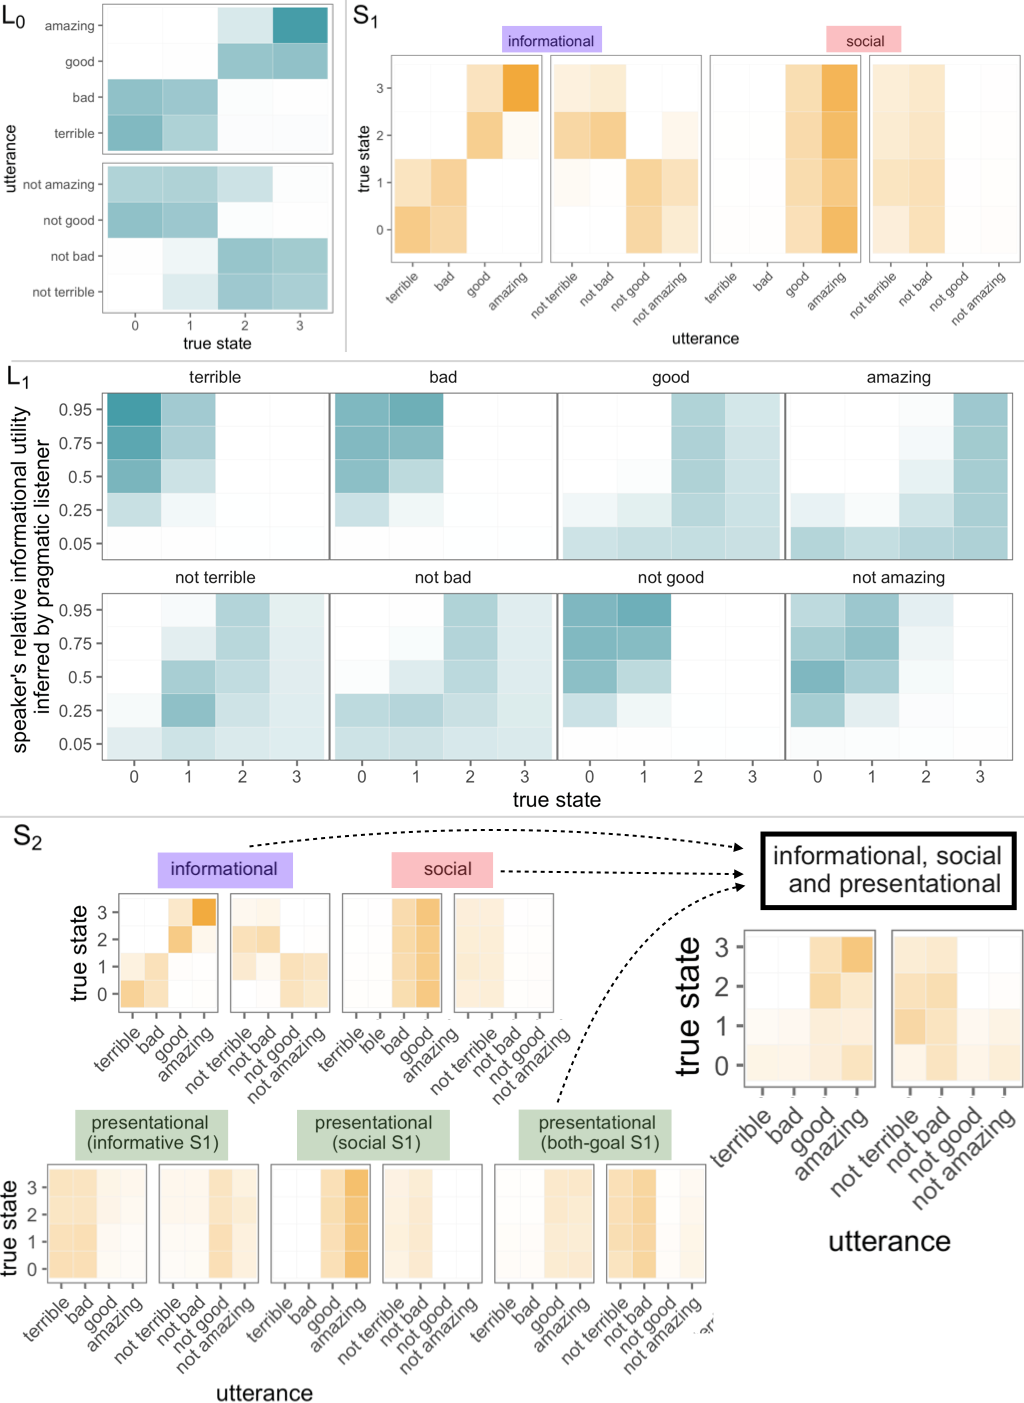
\includegraphics[width=0.8\linewidth]{fig/schematic}}


\caption[Model overview with schematic predictions]{Model overview with schematic predictions. Color saturation indicates probability (listener models) or utility (speaker models). Top left ($L_0$): Literal listener posterior probability distribution over the true state $s$ (x-axis) given utterances (y-axis). Top right ($S_1$): the first-order speaker’s utility of utterances $w$ (x-axis) for different states $s$ (y-axis) given either the informational ($\phi = 1$) or social goal ($\phi = 0$; facets). Informational utility tracks the literal meanings and varies by true state; social utility favors utterances that signal higher valued states. Middle ($L_1$): Politeness-aware listener’s joint posterior distribution over the true state $s$ (x-axis) and $S_1$ utility weighting $\phi$ (y-axis; higher value indicates greater weight on informational utility) given utterances $w$ (facets). Bottom ($S_2$): Second-order speaker’s utility of utterances (y-axis) for different states (x-axis) and different goals $\omega$ (facets). Informational utility tracks the literal meanings and varies by true state; social utility favors utterances that signal high-valued states; three versions of self-presentational utility are shown, corresponding to whether the speaker wants to project informativeness ($\phi = 1$), kindness ($\phi = 0$), or a balance ($\phi = 0.3$). Only the balanced self-presentational speaker shows a preference for indirect speech. The right-most facet shows $S_2$’s utterance preferences when they want to balance all three utilities (informational, social, and presentational to project informativeness and kindness).}\label{fig:schematicPredictionsFig}
\end{figure}

\newpage

The first-order speaker \(S_1\) chooses utterances given a utility
function with two components defined in terms of the literal listener:
informational and social utility. \emph{Informational utility}
(\(U_{inf}\)) is the amount of information about the world state
conveyed to the literal listener \(L_0\) by the utterance \(w\); for
example, the highest information utterance associated with the 2-heart
state is \enquote{good}; the best way to describe the 0-heart state is
\enquote{terrible} (Figure 2, top right; left facet). \emph{Social
utility} (\(U_{soc}\)) is the expected subjective utility of the world
state inferred by the literal listener \(L_0\) given the utterance
\(w\), which does not depend on the true state.\footnote{The
  independence between true state and social utility stems from the
  assumption of no shared beliefs between speaker and listener about the
  true state (i.e., the speaker knows the true state and the listener's
  priors are independent of the true state). This independence is a
  deliberate feature of our experimental setup, designed to best
  disambiguate the models proposed. In future work, it would be
  important to examine how shared beliefs about the true state may
  influence the speaker's utterance choice.} For instance, the highest
social utility utterance is \enquote{amazing}, because it strongly
implies that the listener is in the 3-heart state; negated negative
utterances like \enquote{not bad} also have some degree of social
utility, because they imply high heart states, albeit less directly
(Figure \ref{fig:schematicPredictionsFig}, top right; right facet). The
speaker combines these utilities assuming some weighting \(\phi\) and
subtracts the cost of the utterance (defined in terms of the length of
the utterance) in order to arrive at an overall utility of an utterance
for a state and a goal-weighting:
\(U(w; s; \phi) = \phi \cdot \ln(P_{L_0}(s \mid w)) + (1 - \phi) \cdot \mathbb{E}_{P_{L_0}(s \mid w)}[V(s)] - C(w).\)
The speaker then chooses utterances \(w\) softmax rationally given the
state \(s\) and his goal weight mixture \(\phi\):

\begin{equation}
P_{S_1}(w \mid s, \phi) \propto \mathrm{exp}[\alpha \cdot U[s; w; \phi]]
\end{equation}

The pragmatic listener model \(L_1\) reasons jointly about both the true
state of the world and the speaker's goals (Fig.
\ref{fig:schematicPredictionsFig}, middle). Upon hearing {[}Your poem
was{]} \enquote{amazing}, the listener faces a tough credit-assignment
problem: The poem could indeed be worthy of three hearts, but it is also
possible that the speaker had strong social goals and then no inference
about the quality of the poem is warranted. Hearing {[}Your poem{]} was
\enquote{terrible}, the inference is much easier: the poem is probably
truly terrible (i.e., worthy of zero hearts) and the speaker probably
does not have social goals. Negation makes the interpreted meanings less
precise and hence, inferences about goals are also fuzzier: \enquote{not
amazing} can be seen as a way of saying that the poem was worthy of 0 or
1 hearts, which satisfies some amount of both social and informational
goals. \enquote{Not bad} is less clear: the speaker could be being nice
and the poem was actually worthy of 0- or 1-hearts (i.e., it was bad) or
the speaker could be being honest (i.e., it was not bad) and the poem
was worth 2-hearts.

The second-order pragmatic speaker model (\(S_2\)) reasons about the
pragmatic listener \(L_1\) to decide which utterances to produce based
on both the true state of the world and the speaker's goals (Figure
\ref{fig:schematicPredictionsFig}, bottom). The informational and social
utilities of the second-order speaker mirror those of the first-order
speaker: Direct utterances are more informative than those involving
negation, and utterances that signal many hearts are more
prosocial.\footnote{The second-order speaker's informational utilities
  take into account the listener's pragmatic inferences about the
  speaker's goals. This only really affects the utility of \enquote{not
  terrible}, which has higher information for the 1-heart state because
  the pragmatic listener strongly infers that the utterance was produced
  for social reasons. That is, for the second-order speaker, the
  utterance \enquote{not terrible} is loaded in a way that other
  utterances are not. An alternative formulation could be proposed by
  having \(S_2\)'s informational utility derived from a pragmatic
  listener who doesn't reason about the speaker's goals (i.e., it
  compares a posterior on states assuming the speaker was being
  informative, while independently reasoning about whether the speaker
  was being informative). An examination of this model is beyond the
  scope of this paper.} The interesting novel behavior of this level of
recursion comes from the different flavors of the self-presentational
goal (Figure \ref{fig:schematicPredictionsFig}, bottom). When the
second-order pragmatic speaker wants to \emph{project} kindness (i.e.,
appear prosocial) they even more strongly display the preference for
utterances that signal positive states (i.e., they are over-the-top
positive). When the speaker wants to project honesty and
informativeness, they take the exact opposite strategy, producing
utterances that cannot be explained by virtue of social utility: direct,
negative utterances (e.g., \enquote{it was terrible}). Finally, the
speaker may present themselves in more subtle ways (e.g., intending to
convey they are both kind and honest): This goal uniquely leads to the
indirect, negative utterances (e.g., \enquote{not terrible},
\enquote{not bad}) having high utility. These utterances are literally
incompatible with low-heart states, but are also not highly informative;
this unique combination is what gives rise to the subtle inference of a
speaker who cares about both goals.


\section{Experiment: Speaker production
task}\label{experiment-speaker-production-task}

We conducted a direct test of our speaker production model and its
performance in comparison to a range of alternative models, by
instantiating our running example in an online experiment. We developed
the preceding model iteratively on the basis of a sequence of similar
experiments, but importantly, the current test was fully pre-registered
and confirmatory. All data analytic models and our full model comparison
approach were registered ahead of time to remove any opportunities for
overfitting the behavioral data through changes to the model or the
evaluation.

\begin{figure}[!h]

{\centering 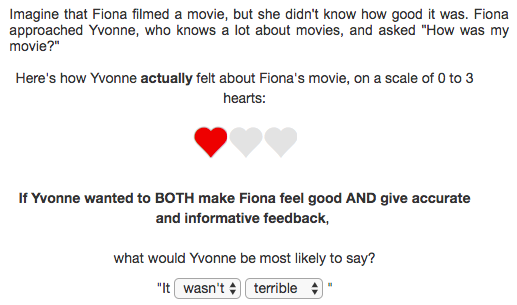
\includegraphics[width=0.7\linewidth]{fig/screenshot} 

}

\caption{Example of a trial in the speaker production task.}\label{fig:screenshot}
\end{figure}

\subsection{Participants}\label{participants}

202 participants with IP addresses in the United States were recruited
on Amazon's Mechanical Turk.

\subsection{Design and Methods}\label{design-and-methods}

Participants read scenarios with information on the speaker's feelings
toward some performance or product (e.g., a poem recital), on a scale
from zero to three hearts (e.g., one out of three hearts; \emph{true
state}). For example, one trial read: \emph{Imagine that Bob gave a poem
recital, but he didn't know how good it was. Bob approached Ann, who
knows a lot about poems, and asked} \enquote{How was my poem?}
Additionally, we manipulated the speaker's goals across trials: to be
\emph{informative} (\enquote{give accurate and informative feedback});
to be \emph{kind} (\enquote{make the listener feel good}); or to be
\emph{both} informative and kind simultaneously. Notably, we did not
mention a self-presentational goal to participants; rather, we
hypothesize this goal would arise spontaneously from a speaker's
inability to achieve the first-order goals of niceness and honesty
(i.e., if a speaker wants to, but can't, be both honest and nice, they
would instead try to signal that they care about both goals). We
hypothesized that each of the three experimentally-induced goals
(\emph{informative}, \emph{kind}, \emph{both}) would induce a different
tradeoff between the informational, prosocial, and self-presentational
utilities in our model.

Each participant read twelve scenarios, depicting every possible
combination of the three goals and four states. The order of context
items was randomized, and there were a maximum of two repeats of each
context item per participant. In a single trial, each scenario was
followed by a question that read, \enquote{If Ann wanted to make Bob
feel good but not necessarily give informative feedback (or to give
accurate and informative feedback but not necessarily make Bob feel
good, or BOTH make Bob feel good AND give accurate and informative
feedback), what would Ann be most likely to say?} Participants indicated
their answer by choosing one of the options on the two dropdown menus,
side-by-side, one for choosing between \emph{It was} vs. \emph{It
wasn't} and the other for choosing among \emph{terrible}, \emph{bad},
\emph{good}, and \emph{amazing} (Figure \ref{fig:screenshot}).

\subsection{Behavioral results}\label{behavioral-results}

\begin{figure}[!h]
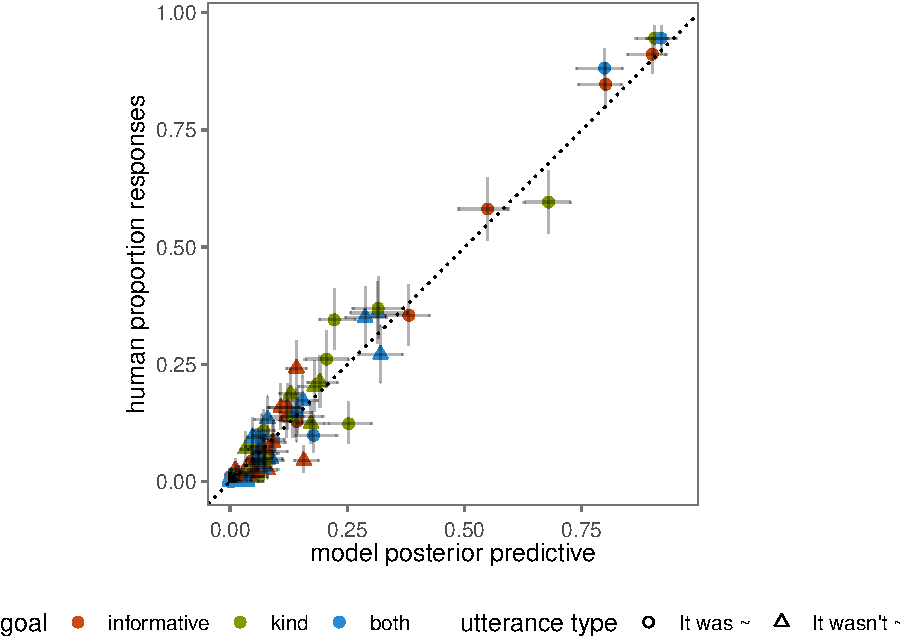
\includegraphics[width=\textwidth]{polite_manuscript_files/figure-latex/variance-1} \caption{Full distribution of human responses vs. model predictions. Error bars represent 95\% confidence intervals for the data (vertical) and 95\% highest density intervals for the model (horizontal).}\label{fig:variance}
\end{figure}

Our primary behavioral hypothesis was that speakers describing bad
states (e.g., a poem deserving 0 hearts) with goals to be both
informative and kind would produce more indirect, negative utterances
(e.g., \emph{It wasn't terrible}). Such indirect speech acts both save
the listener's face and provide some information about the true state,
and thus, are what a socially-conscious speaker would say (Figure
\ref{fig:schematicPredictionsFig}, bottom). This prediction was
confirmed, as a Bayesian mixed-effects model predicts more negation as a
function of true state and goal via an interaction: A speaker with both
goals to be informative and kind produced more negation in worse states
compared to a speaker with only the goal to be informative (posterior
mean \emph{M} = -1.33, with 95\% Bayesian credible interval of {[}-1.69,
-0.98{]}) and goal to be kind (\emph{M} = -0.50, {[}-0.92, -0.07{]}).
Rather than eschewing one of their goals to increase utility along a
single dimension, participants chose utterances that jointly satisfied
their conflicting goals by producing indirect speech.

\subsection{Model results}\label{model-results}

\begin{figure}[!h]
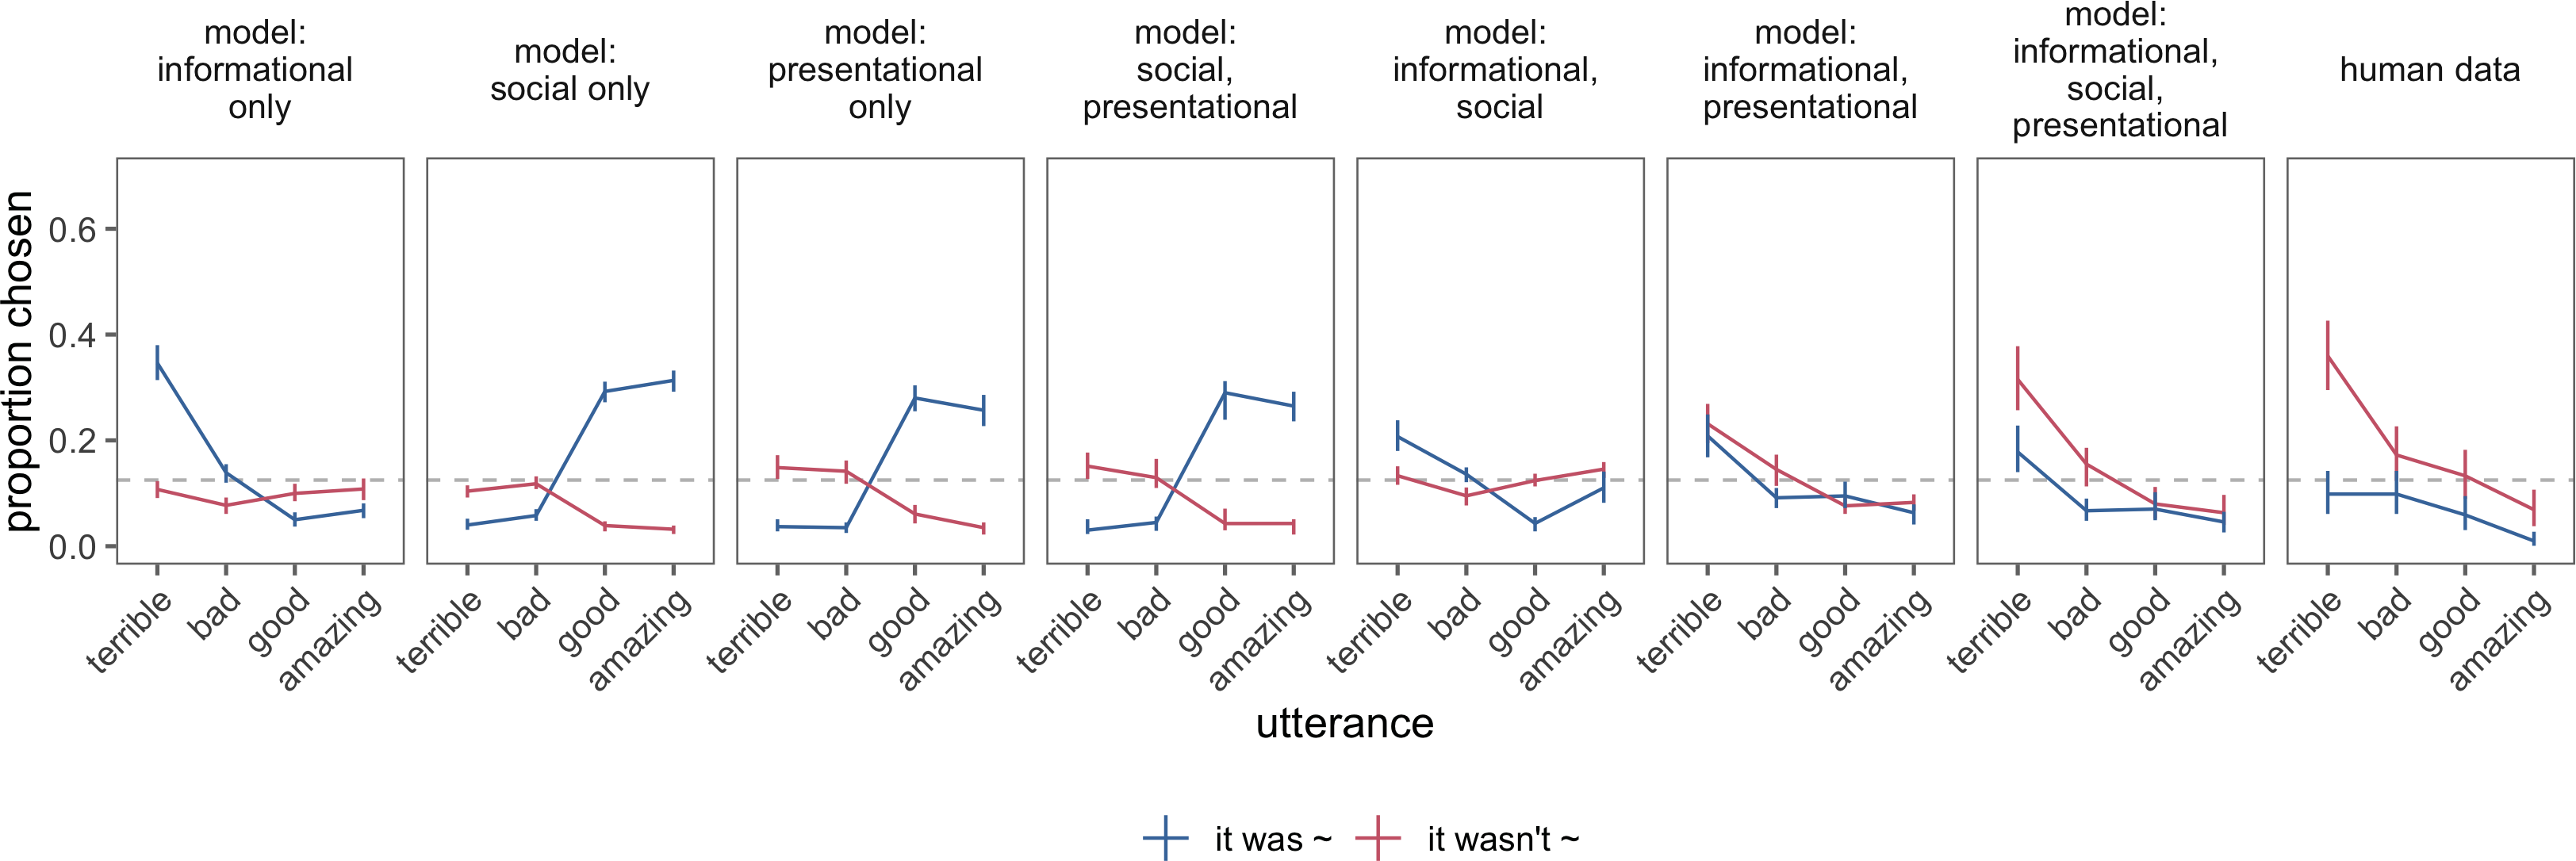
\includegraphics[width=\textwidth]{polite_manuscript_files/figure-latex/comparison-1} \caption{Comparison of predictions for proportion of utterances chosen by pragmatic speaker from possible model variants (left) and human data (rightmost) for average proportion of negation produced among all utterances, given true state of 0 heart (on a scale of 0 to 3) and speaker with both goals to be informative and kind. Gray dotted line indicates chance level at 12.5\%.}\label{fig:comparison}
\end{figure}

\begin{table}[tbp]
\begin{center}
\begin{threeparttable}
\caption{\label{tab:phi}Inferred goal weight ($\omega_g$) and speaker-projected informativity-niceness weight ($\phi$) parameters from all model variants with more than one utility.}
\begin{tabular}{llllll}
\toprule
model (utilities) & \multicolumn{1}{c}{goal} & \multicolumn{1}{c}{$\omega_{inf}$} & \multicolumn{1}{c}{$\omega_{soc}$} & \multicolumn{1}{c}{$\omega_{pres}$} & \multicolumn{1}{c}{$\phi$}\\
\midrule
informational, social, presentational & both & 0.36 & 0.11 & 0.54 & 0.36\\
informational, social, presentational & informative & 0.36 & 0.02 & 0.62 & 0.49\\
informational, social, presentational & social & 0.25 & 0.31 & 0.44 & 0.37\\
informational, presentational & both & 0.64 & -- & 0.36 & 0.17\\
informational, presentational & informative & 0.77 & -- & 0.23 & 0.33\\
informational, presentational & social & 0.66 & -- & 0.34 & 0.04\\
informational, social & both & 0.54 & 0.46 & -- & --\\
informational, social & informative & 0.82 & 0.18 & -- & --\\
informational, social & social & 0.39 & 0.61 & -- & --\\
social, presentational & both & -- & 0.38 & 0.62 & 0.55\\
social, presentational & informative & -- & 0.35 & 0.65 & 0.75\\
social, presentational & social & -- & 0.48 & 0.52 & 0.66\\
\bottomrule
\end{tabular}
\end{threeparttable}
\end{center}
\end{table}

\begin{figure}[!h]

{\centering 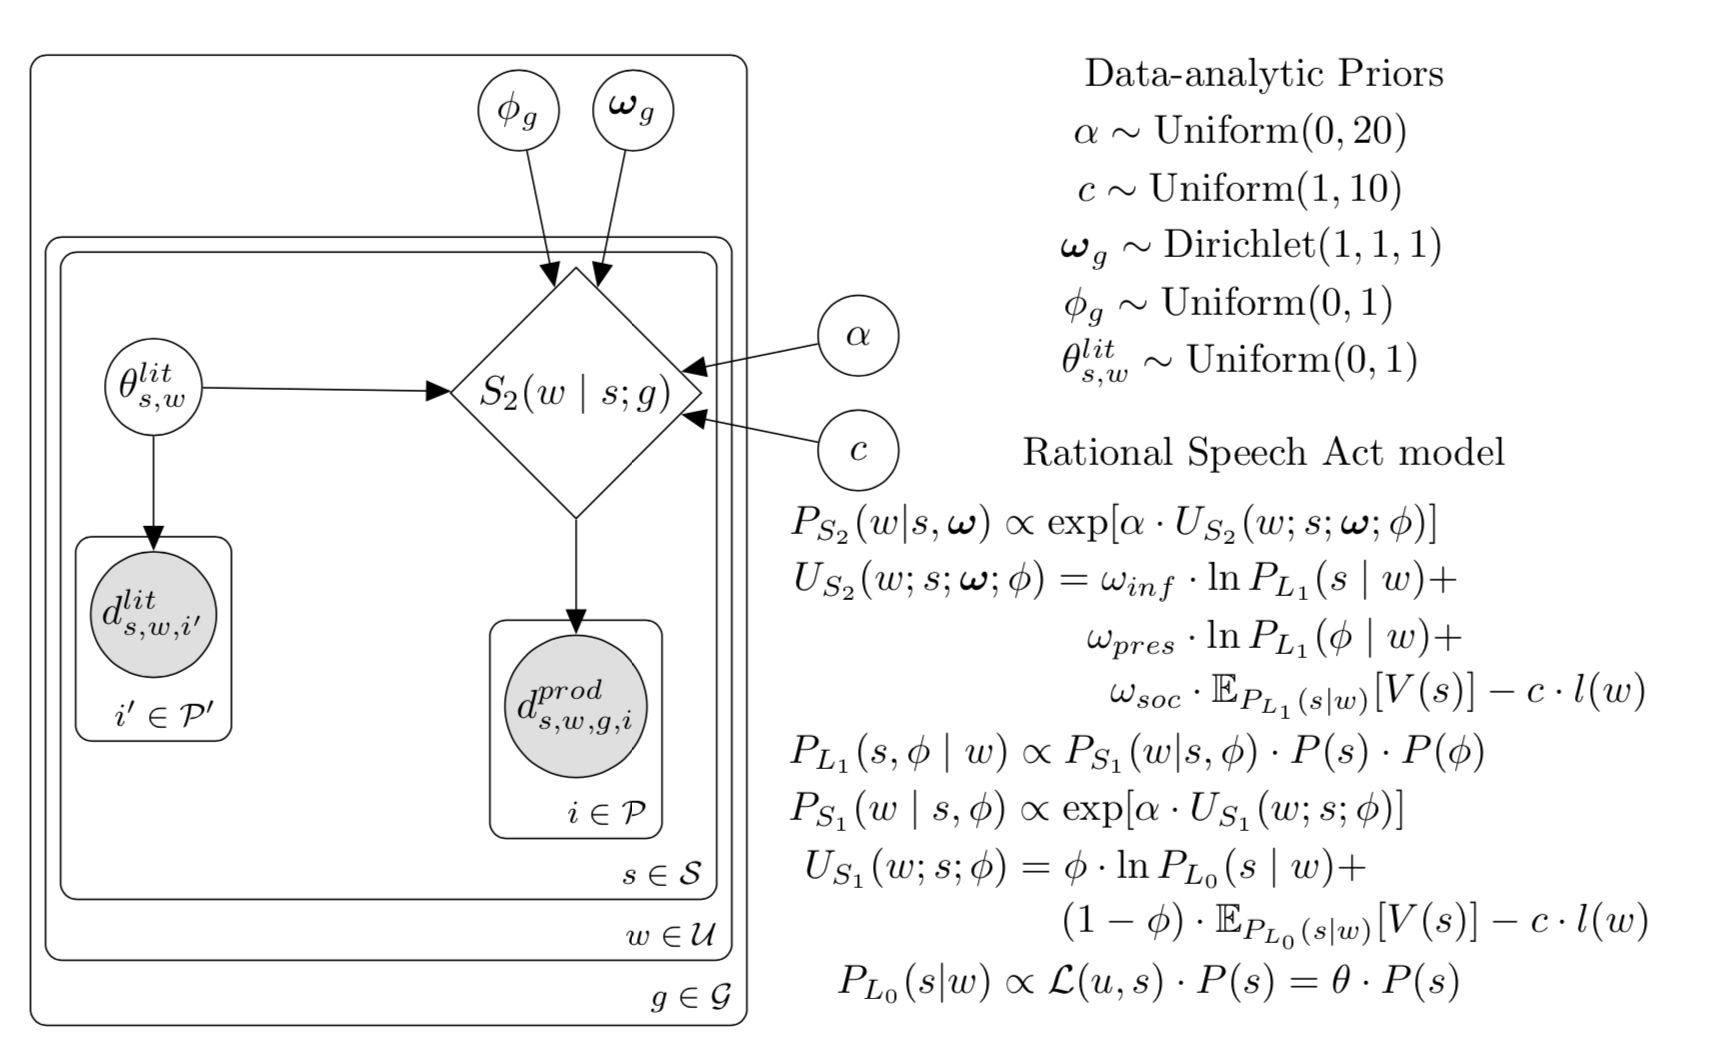
\includegraphics[width=0.7\linewidth]{fig/bayesnet} 

}

\caption{Graphical model representing our Bayesian data analytic approach for the full 3-component model (other models contain subsets of the parameters shown). $S_2$ represents the RSA speaker model defined by Eq. 1, which is used to predict the production responses $d^{prod}$ of each participant $i$, for each state $s$ (number of hearts), for each utterance $w$, in each goal condition $g$. The RSA speaker model takes as input the literal meaning variables $\theta$, which additionally are used to predict the literal meaning judgments $d^{lit}$ assuming a Bernoulli linking function. Additionally, the RSA model takes the speaker’s goal weights $\omega$ and intended presentational goal weight $\phi$, which are inferred separately for each goal condition $g$. Finally, the RSA model uses two global free parameters: the cost of negation $c$ (or, utterance length $l$ in terms of number of words) and the speaker’s rationality parameter $\alpha$. Minimally-assumptive priors over parameters shown in top-right.}\label{fig:bayesnet}
\end{figure}

\begin{table}[tbp]
\begin{center}
\begin{threeparttable}
\caption{\label{tab:comparisonTable}Comparison of variance explained for each model variant and log Bayes Factors quantifying evidence in favor of alternative model in comparison.}
\begin{tabular}{lll}
\toprule
model & \multicolumn{1}{c}{variance 
explained} & \multicolumn{1}{c}{log BF}\\
\midrule
informational, 
social, 
presentational & 0.97 & --\\
informational, 
presentational & 0.96 & -11.14\\
informational, 
social & 0.92 & -25.06\\
social, 
presentational & 0.23 & -864\\
presentational 
only & 0.23 & -873.83\\
social only & 0.22 & -885.52\\
informational 
only & 0.83 & -274.89\\
\bottomrule
\end{tabular}
\end{threeparttable}
\end{center}
\end{table}


We assume our experimental goal conditions (informative vs.~kind
vs.~both) induce a set of weights over the utilities
\(\boldsymbol{\omega}\) in participants' utterance production model. In
addition, the self-presentational utility is defined via a communicated
social weight \(\phi\) (i.e., the mixture of informative vs.~social that
the speaker is trying to project). The mapping from social situations
into utility weights and communicated social weight is a complex
mapping, which we do not attempt to model here; instead, we infer these
parameters for each goal condition from the data. We additionally infer
the literal meanings (i.e., the semantics) of the words as interpreted
by the literal listener \(L_0\) with the additional constraint of the
literal meaning judgments from an independent group of participants (See
Supplementary Materials: Literal semantic task section). Finally, the
RSA model has two global free parameters: the softmax speaker optimality
\(\alpha\) and utterance cost of negation \(c\), which we infer from the
data (Figure \ref{fig:bayesnet}). We implement this data analytic model
for each of the alternative models and infer the parameters using
Bayesian statistical inference \citep{lee2014}. We use
uninformative priors over ranges consistent with the prior literature on
RSA models: \(\theta_{s,w}^{lit} \sim \text{Uniform}(0, 1)\),
\(\phi_g \sim \text{Uniform}(0, 1)\),
\(\boldsymbol{\omega}_g \sim \text{Dirichlet}(1,1,1)\),
\(\alpha \sim \text{Uniform}(0, 20)\), \(c \sim \text{Uniform}(1, 10)\).
This analysis tells us which, if any, of these models can accomodate all
of the patterns in the empirical data. The posterior predictions from
the three-utility polite speaker model (informational, social,
presentational) showed a very strong fit to participants' actual
utterance choices (\(r^2\)(96) = 0.97; Figure \ref{fig:variance}). Other
models (e.g., informational + presentational), however, show comparably
high correlations to the full data set; correlations can be inflated
through the presence of many 0s (or 1s) in the data set, which our data
contains since certain utterance choices are implausible given a
particular state and goal condition. Thus, we compare model variants
using a bonafide model comparison technique, Bayes Factors, which
balance predictive accuracy with model complexity in quantifying the
goodness of fit of a model.

Bayes Factors compare the likelihood of the data under each model,
averaging over the prior distribution of the model parameters; by
averaging over the prior distribution over parameters, Bayes Factors
penalize models with extra flexibility because increasing the
flexibility of the model to fit more data sets decreases the average fit
of the model to a particular data set \citep{lee2014},
capturing the intuition that a theory that can predict anything predicts
nothing. That is, simply because a model has more parameters and can
explain more of the variance in the data set does not entail that it
will assign the highest marginal likelihood to the actual data. Here,
however, both the variance explained and marginal likelihood of the
observed data were the highest for the full model: The full model was at
least 5 x \(10^4\) times better at explaining the data than the next
best model (Table \ref{tab:comparisonTable}). Only the full model
captured participants' preference for negation when the speaker wanted
to be informative and kind about truly bad states, as hypothesized
(Figure \ref{fig:comparison}). In sum, the full set of informational,
social, and presentational utilities were required to fully explain
participants' utterance choices.

The utility weights inferred for the three-utility model (Table
\ref{tab:phi}) provide additional insight into how polite language use
operates in our experimental context and possibly beyond. As expected,
the weight on social utility (\(\omega_{soc}\)) is highest when the
speaker is trying to \emph{be kind} and lowest when the speaker is
\emph{being informative}. Informational utility (\(\omega_{inf}\)) is
highest when the goal is to be informative or \emph{informative and
kind} (\enquote{both goal}). The weight on projecting kindness
(\(\omega_{pres}\)) is also highest for the \emph{informative} and the
\emph{both-goal} conditions, though the degree of kindness being
projected (\(\phi\)) varies between these conditions: A greater degree
of kindness is projected in the \emph{both-goal} relative to the
\emph{informative} condition. In all conditions, however, the
presentational utility has a high weight, suggesting that managing the
listener's inferences about oneself was integral to participants'
decisions in the context of our communicative task. Overall then, our
condition manipulation altered the balance between these weights, but
all utilities played a role in all conditions.

\section{Discussion}\label{discussion}

Politeness is puzzling from an information-theoretic perspective.
Incorporating social motivations into theories of language use adds a
level of explanation, but so far such intuitions and observations have
resisted both formalization and precise testing. We presented a set of
utility-theoretic models of language use that captured different
proposals about the interplay between competing informational, social,
and presentational goals. Our full model instantiated a novel
theoretical proposal, namely that indirect speech is a response to the
conflict between informational and social utilities that preserves
speakers' self-presentation. Our confirmatory test of the comparison
between these models then provided experimental evidence that the full
model best fit participants' judgments, even accounting for differences
in model complexity.

The most substantial innovation in our full model is the formalization
of a self-presentational utility, defined only for a speaker who reasons
about a listener who reasons about a speaker. We hypothesized that a
speaker who prioritizes presentational utility will tend to produce more
indirect speech (negation in our experimental paradigm). Indeed, this is
consistent with previous work showing that people prefer to use negation
(\enquote{that's not true} as opposed to \enquote{that's false}) when
prompted to speak more \enquote{politely} \citep{giora2005} and that utterances involving negation tend to be
interpreted in a more mitigated and hedged manner compared to direct
utterances \citep{colston1999}. It also may help explain the
phenomenon of negative strengthening, where negation of a positive
adjective can be interpreted in a rather negative manner \citep[e.g., ``He's
not brilliant'' meaning ``he is rather unintelligent''; ][]{gotzner2018, horn1989}. Our work builds on this previous work that
shows a preference for negation by elucidating the goal-directed
underpinnings of this behavior and possible contextual modulation of
this preference. An interesting open question is whether other
negation-related politeness phenomena \citep[e.g., indirect questions such as
``You couldn't possibly tell me the time, could you?''; ][]{brown1987} can be derived from the basic information-theoretic
goals we formalize.

In order to conduct quantitative model comparisons, we needed to create
an experiment with repeated trials and a restricted range of choices.
Thus, we had to abstract away from the richness of natural interactions.
These choices decrease the validity of our experiment. Despite these
abstractions, we showed that behavior in the experiment reflected social
and informational pressures described in previous theories of polite
language, providing some face validity to the responses we collected.
With a formal model in hand, it now will be possible to consider
relaxing some of the experimental simplifications we put into place in
future work. Most importantly, human speakers have access to a
potentially infinite set of utterances to select from in order to manage
the politeness-related tradeoffs (e.g., \emph{It's hard to write a good
poem}, \emph{That metaphor in the second stanza was so relatable!}).
Each utterance will have strengths and weaknesses relative to the
speaker's goals. Computation in an unbounded model presents technical
challenges (perhaps paralleling the difficulty human speakers feel in
finding the right thing to say in a difficult situation), and addressing
these challenges is an important future direction \citep[see ][]{goodman2016}.

For a socially-conscious speaker, managing listeners' inferences is a
fundamental task. Our work extends previous models of language beyond
standard informational utilities to address social and
self-presentational concerns. Further, our model builds upon the theory
of politeness as face management \citep{brown1987} and takes a
step towards understanding the complex set of social concerns involved
in face management. This latter point illustrates a general feature of
why explicit computational models provide value: only by formalizing the
factors in \citet{brown1987}'s theory were we able to recognize
that they were an insufficient description of the data we were
collecting in previous versions of the current experiment. Those
failures allowed us to explore models with a broader range of utilities,
such as the one reported here.

Previous game-theoretic analyses of politeness have either required some
social cost to an utterance \citep[e.g., by reducing one's social status or
incurring social debt to one's conversational partner; ][]{vanRooy2003} 
or a separately-motivated notion of plausible deniability \citep{pinker2008}. 
The kind of utterance cost for the first type of
account would necessarily involve higher-order reasoning about other
agents, and may be able to be defined in terms of the more basic social
and self-presentational goals we formalize here. A separate notion of
plausible deniability may not be needed to explain most politeness
behavior, either. Maintaining plausible deniability is in one's own
self-interest (e.g., due to controversial viewpoints or covert
deception) and goes against the interests of the addressee; some amount
of utility dis-alignment is presumed by these accounts. Politeness
behavior appears present even in the absence of obvious conflict,
however: In fact, you might be even more motivated to be polite to
someone whose utilities are more aligned with yours (e.g., a friend). In
our work here, we show that such behaviors can in fact arise from purely
cooperative goals \citep{brown1987}, though in cases of genuine
conflict, plausible deniability likely plays a more central role in
communication. Our computational model is also closely related to recent
developments in modeling \enquote{social meaning} in sociolinguistics,
where a speaker chooses how they say something (e.g., \enquote{I'm
grilling} vs. \enquote{I'm grillin'}) in order to convey something about
themselves (e.g., social class) to the listener \citep{burnett2019}. Unlike
a Social Meaning Game which treats properties of a speaker as
first-class targets of communication, our model considers the properties
of the speaker as variables that modify the speaker's utility function,
about which the listener can then reason \citep[but see also: ][]{henderson2019, qing2019}.

Utility weights and value functions in our model could provide a
framework for a quantitative understanding of systematic cross-cultural
differences in what counts as polite. Cultures may place value on
satisfying different communicative goals, and speakers in these cultures
may pursue those goals more strongly than speakers from other cultures.
For example, we found in our model that a speaker who wants to appear
informative should speak more negatively than a truly informative
speaker; one could imagine run-away effects where a group becomes overly
critical from individuals' desires to appear informative. Culture could
also affect the value function \(V\) that maps states of the world onto
subjective values for the listener. For example, the mapping from states
to utilities may be nonlinear and involve reasoning about the future; a
social utility that takes into account reasoning about the future could
help explain why it can often be nice to be informative. Our formal
modeling approach, with systematic behavior measurements, provides an
avenue towards understanding the vast range of politeness practices
found across languages and contexts \citep{katz2005}.

Politeness is only one of the ways language use deviates from purely
informational transmission. We flirt, insult, boast, and empathize by
balancing informative transmissions with goals to affect others'
feelings or present particular views of ourselves. Our work shows how
social and self-presentational motives can be integrated with
informational concerns more generally, opening up the possibility for a
broader theory of social language. A formal account of politeness may
also move us closer to courteous computation -- to machines that can
talk with tact.


\section{Supplementary Materials}\label{supplementary-materials}

\subsection{Model details}\label{model-details}

The full, three-component utility model is given by the following set of
equations.

\begin{align}
P_{L_0}(s | w) &\propto \mathcal{L}(u, s) \cdot P(s)\label{eq:L0} \\ 
P_{S_1}(w \mid s, \phi) &\propto \mathrm{exp}[\alpha \cdot ( \phi \cdot \ln P_{L_0}(s \mid w) + (1 - \phi) \cdot \mathbb{E}_{P_{L_0}(s \mid w)}[V(s)] - C(w))] \label{eq:S1}  \\ 
P_{L_1}(s, \phi | w) &\propto P_{S_1}(w | s, \phi) \cdot P(s) \cdot P(\phi)  \label{eq:L1a} \\
P_{S_2}(w | s, \boldsymbol{\omega}) &\propto \exp[\alpha \cdot (\omega_{inf} \cdot \ln P_{L_1}(s \mid w) + \omega_{soc} \cdot \mathbb{E}_{P_{L_1}(s \mid w)}[V(s)] + \omega_{pres} \cdot P_{L_1}(\phi \mid w) - C(w) )] \label{eq:S2a} 
\end{align}

The \emph{literal listener} \(L_0\) (Eq. \ref{eq:L0}) is a simple
Bayesian agent that takes the utterance \(w\) to be true to update a
prior distribution over world states \(P(s)\) and return a posterior
distribution over states \(P_{L_0}(s | w)\). We assume the prior over
world states is uninformative and thus Eq. \ref{eq:L0} reduces to
\(P_{L_0}(s | w) \propto \mathcal{L}(u, s)\).
\(\mathcal{L}(u, s) = \theta \in [0,1]\) denotes a continuously-valued
lexicon where \(\theta\) is the probability that the utterance \(u\) is
true of state \(s\); this kind of lexicon is a generalization of the
more traditional, binary truth functional semantics \citep[see ][ for a discussion of this kind of
\enquote{soft semantics}]{degen2020}. \(\theta\) is estimated empirically from the
Literal Semantics task described in the next section, where it is
roughly the proportion of participants who endorse the utterance \(u\)
in state \(s\) in the Literal Semantics task.

The first-order \emph{speaker} \(S_1\) (Eq. \ref{eq:S1}) chooses
utterances approximately optimally given a utility function, which can
be decomposed into two components: informational and social utility.
First, informational utility (\(U_{inf}\)) is the amount of information
a literal listener \(L_0\) would still not know about world state \(s\)
after hearing a speaker's utterance \(w\), and is given by the log
probability of the world state given the utterance \(\ln P(s \mid w)\).
Second, social utility (\(U_{soc}\)) is the expected subjective utility
of the state inferred given the utterance \(w\):
\(\mathbb{E}_{P_{L_0}(s \mid w)}[V(s)]\), where \(V(s)\) denotes the
subjective utility function that maps states of the world \(s\) onto
subjective values. For this paper, we assume that \(V\) is the identity
function that returns the number of hearts which defines a state. The
overall utility of an utterance subtracts the cost \(c(w)\) from the
weighted combination of the social and informational utilities, and the
speaker then chooses utterances \(w\) softmax-optimally given the state
\(s\) and his goal weight mixture \(\phi\).

Equations \ref{eq:L1a} and \ref{eq:S2a} are described in the main text.
Eq. \ref{eq:L1a} is a model of a pragmatic listener who jointly reasons
about the state of the world and the first-order speaker's utility
weighting (social vs.~informational utility). Again, we assume an
uninformative prior over states as well as an uninformed prior over the
speakear's utility weights. Eq. \ref{eq:S2a} is a model of a
second-order pragmatic speaker who produces utterances approximately
optimally given a three-component utility function: informational,
social, and presentational utilities. These utilities are defined with
respect to the pragmatic listener \(L_1\) and are computed by
marginalizing \(L_1\)'s joint distribution over states and
utility-weights:
\(P_{L_1}(s | w) = \int_\phi P_{L_1}(s, \phi | w) d\phi\) and
\(P_{L_1}(\phi | w) = \int_s P_{L_1}(s, \phi | w) ds\). The definitions
of social and informational utility mirror those of the first-order
speaker, only they are defined with respect to the \(L_1\) distribution
as opposed to the \(L_0\) distribution. The self-presentational utility
is the negative surprisal of the goal-weight parameter that \(L_1\)
reasons about: \(\ln P_{L_1}(\phi | w)\). These three utilities are then
weighed by a set of three mixture components \(\boldsymbol{\omega}\),
which are inferred from the data separately for each experimental
condition (see main text for details).

\subsection{Literal semantics task}\label{literal-semantics-task}

We probed judgments of literal meanings of the target words assumed by
our model and used in our main experiment.

\subsubsection{Participants}\label{participants-1}

51 participants with IP addresses in the United States were recruited on
Amazon's Mechanical Turk.

\subsubsection{Design and Methods}\label{design-and-methods-1}

We used thirteen different context items in which a speaker evaluated a
performance of some kind. For example, in one of the contexts, Ann saw a
presentation, and Ann's feelings toward the presentation (true state)
were shown on a scale from zero to three hearts (e.g., two out of three
hearts filled in red color; see Figure~\ref{fig:screenshot} for an
example of the heart scale). The question of interest was \enquote{Do
you think Ann thought the presentation was / wasn't X?} and participants
responded by choosing either \enquote{no} or \enquote{yes.} The target
could be one of four possible words: \emph{terrible}, \emph{bad},
\emph{good}, and \emph{amazing}, giving rise to eight different possible
utterances (with negation or no negation). Each participant read 32
scenarios, depicting every possible combination of states and
utterances. The order of context items was randomized, and there were a
maximum of four repeats of each context item per participant.

\subsubsection{Behavioral results}\label{behavioral-results-1}

We analyzed the data by collapsing across context items. For each
utterance-state pair, we computed the posterior distribution over the
semantic weight (i.e., how consistent X utterance is with Y state)
assuming a uniform prior over the weight (i.e., a standard Beta-Binomial
model). Meanings of the words as judged by participants were as one
would expect (Figure \ref{fig:litsem}). Importantly, the task does not
elicit alternative-based pragmatic reasoning that would result in
pragmatically-enriched meanings (e.g., \enquote{good} is interpreted to
mean \enquote{not amazing}; instead \enquote{good} is judged equally
true at 2 and 3 heart states)

\begin{figure}[!h]
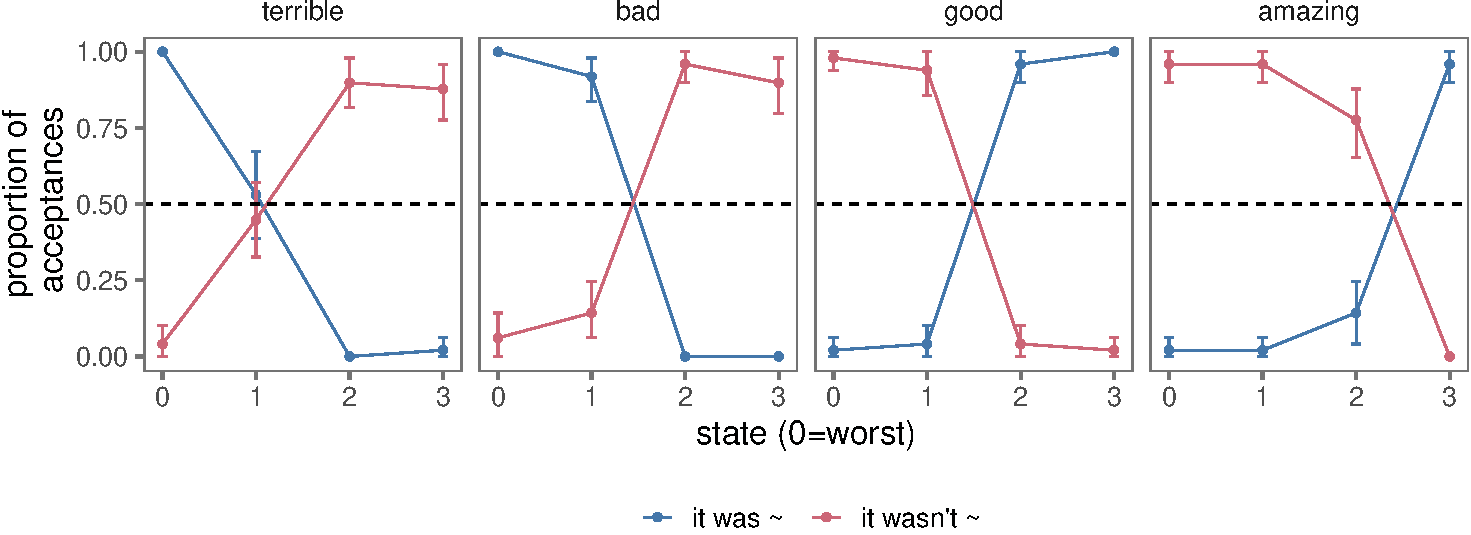
\includegraphics[width=\textwidth]{polite_manuscript_files/figure-latex/litsem-1} \caption{Semantic measurement results. Proportion of acceptances of utterance types (shown in different colors) combined with target words (shown in different facets) given the true state represented on a scale of hearts. Error bars represent 95\% confidence intervals.}\label{fig:litsem}
\end{figure}

\subsection{Full statistics on human
data}\label{full-statistics-on-human-data}

\begin{table}[tbp]
\begin{center}
\begin{threeparttable}
\caption{\label{tab:brmTab}Predictor mean estimates with standard deviation and 95\% credible interval information for a Bayesian linear mixed-effects model predicting negation production based on true state and speaker goal (with both-goal as the reference level).}
\begin{tabular}{lllll}
\toprule
Predictor & \multicolumn{1}{c}{Mean} & \multicolumn{1}{c}{SD} & \multicolumn{1}{c}{95\% CI-Lower} & \multicolumn{1}{c}{95\% CI-Upper}\\
\midrule
Intercept & 0.88 & 0.13 & 0.63 & 1.12\\
True state & 2.18 & 0.17 & 1.86 & 2.53\\
Goal: Informative & 0.47 & 0.17 & 0.14 & 0.80\\
Goal: Kind & 0.97 & 0.25 & 0.51 & 1.49\\
True state * Informative & -1.33 & 0.18 & -1.69 & -0.98\\
True state * Kind & -0.50 & 0.22 & -0.92 & -0.07\\
\bottomrule
\end{tabular}
\end{threeparttable}
\end{center}
\end{table}

We used Bayesian linear mixed-effects models (\texttt{brms} package in
R; Bürkner, 2017) using crossed random effects of true state and goal
with maximal random effects structure \citep{barr2013random, gelman2006data}. The full statistics are shown in Table
\ref{tab:brmTab}.

\subsection{Model fitting and inferred
parameters}\label{model-fitting-and-inferred-parameters}

\begin{table}[tbp]
\begin{center}
\begin{threeparttable}
\caption{\label{tab:otherParams}Inferred negation cost and speaker optimality parameters for all model variants.}
\begin{tabular}{lll}
\toprule
Model & \multicolumn{1}{c}{Cost of negation} & \multicolumn{1}{c}{Speaker optimality}\\
\midrule
informational only & 1.58 & 8.58\\
informational, presentational & 1.89 & 2.93\\
informational, social & 1.11 & 3.07\\
informational, social, presentational & 2.64 & 4.47\\
presentational only & 2.58 & 9.58\\
social only & 1.73 & 7.23\\
social, presentational & 2.49 & 5.29\\
\bottomrule
\end{tabular}
\end{threeparttable}
\end{center}
\end{table}

Other than speaker goal mixture weights explained in the main text
(shown in Table \ref{tab:phi}), the full model has two global
parameters: the speakers' (both \(S_1\) and \(S_2\)) soft-max parameter
\(\alpha\), which we assume to be the same value, and the utterance cost
parameter \(c\). We operationalize utterance cost as a penalty on the
number of words in an utterance; since utterances are only one or two
words long, and two word-long utterances are those involving the
negation particle \enquote{not}, this cost parameter can also be thought
of as a cost of producing a negation particle. We use minimally
assumptive priors that are consistent with those used for similar models
in this model class: \(\alpha \sim \text{Uniform}(0,20)\),
\(c \sim \text{Uniform}(1,10)\). Cost \(c\) is assumed to be greater
than 1; values less than 1 would imply that a two word-long utterance is
cheaper than a one-word long utterance (or, that there is a cost to not
producing negation). Finally, we incorporate the literal semantics data
into the RSA model by maintaining uncertainty about the semantic weight
\(\theta\) of utterance \(w\) for state \(s\), for each of the states
and utterances, and assuming a Beta-Binomial linking function between
these weights and the literal semantics data (see \emph{Literal
Semantics task} above). We infer the posterior distribution over all of
the model parameters and generate model predictions based on this
posterior distribution using Bayesian data analysis \citep{lee2014}. We ran 4 MCMC chains for 80,000 iterations,
discarding the first 40,000 for burnin. The inferred Maximum
A-Posteriori values of parameters are shown in Table
\ref{tab:otherParams}.

We observe that the posterior distributions of the inferred parameters
governing the speaker goal mixture weights are unstable across different
MCMC chains. To confirm these observations, we ran 3 additional MCMC
chains for 350,000 iterations. The resulting posterior distributions for
the utility-weight parameters as a function of the goal condition (a
\enquote{goal-centric} view) are shown in Figure
~\ref{fig:posteriorParamByGoal}. As can be seen by comparing across the
rows of Figure ~\ref{fig:posteriorParamByGoal}, both the values and the
relative orderings of the utility-weight parameters vary as a function
of the chain. For instance, in one run of the model, the informative
goal condition has as its strongest utility weight the presentational
utility (chain 1); in another, the strongest utility weight is the
informational utility (chain 2); in yet another, the informational and
presentational weights are approximately equal in strength (chain 3). At
the same time, for the informative goal condition, the social utility
weight is always close to 0, in all runs of the model. Indeed, the
social utility weight appears most consistent across goal conditions and
chains. Further, when we examine the utility weights as a function of
goal conditions (a \enquote{utility-centric} view), we find other
signatures of consistency (Figure ~\ref{fig:posteriorParamByUtility}).
The relative ordering of goals is consistent across different MCMC
chains; for example, the social-utility weight is highest for the social
goal condition, lowest for the informational goal, and in the middle for
the both-goal condition. In addition, the projected social-utility
weight \(\phi\) is inferred to be more on the informational-side (higher
\(\phi\) value) for the informational goal than for the social or both
goal conditions. These patterns suggest that a lower-dimensional
parameterization of the model may be available, though the posterior
predictive fits and model comparison presented in the main text suggest
that the model's parameterization has the appropriate flexibility
necessary to account for our experimental data.

\begin{figure}[!h]

{\centering 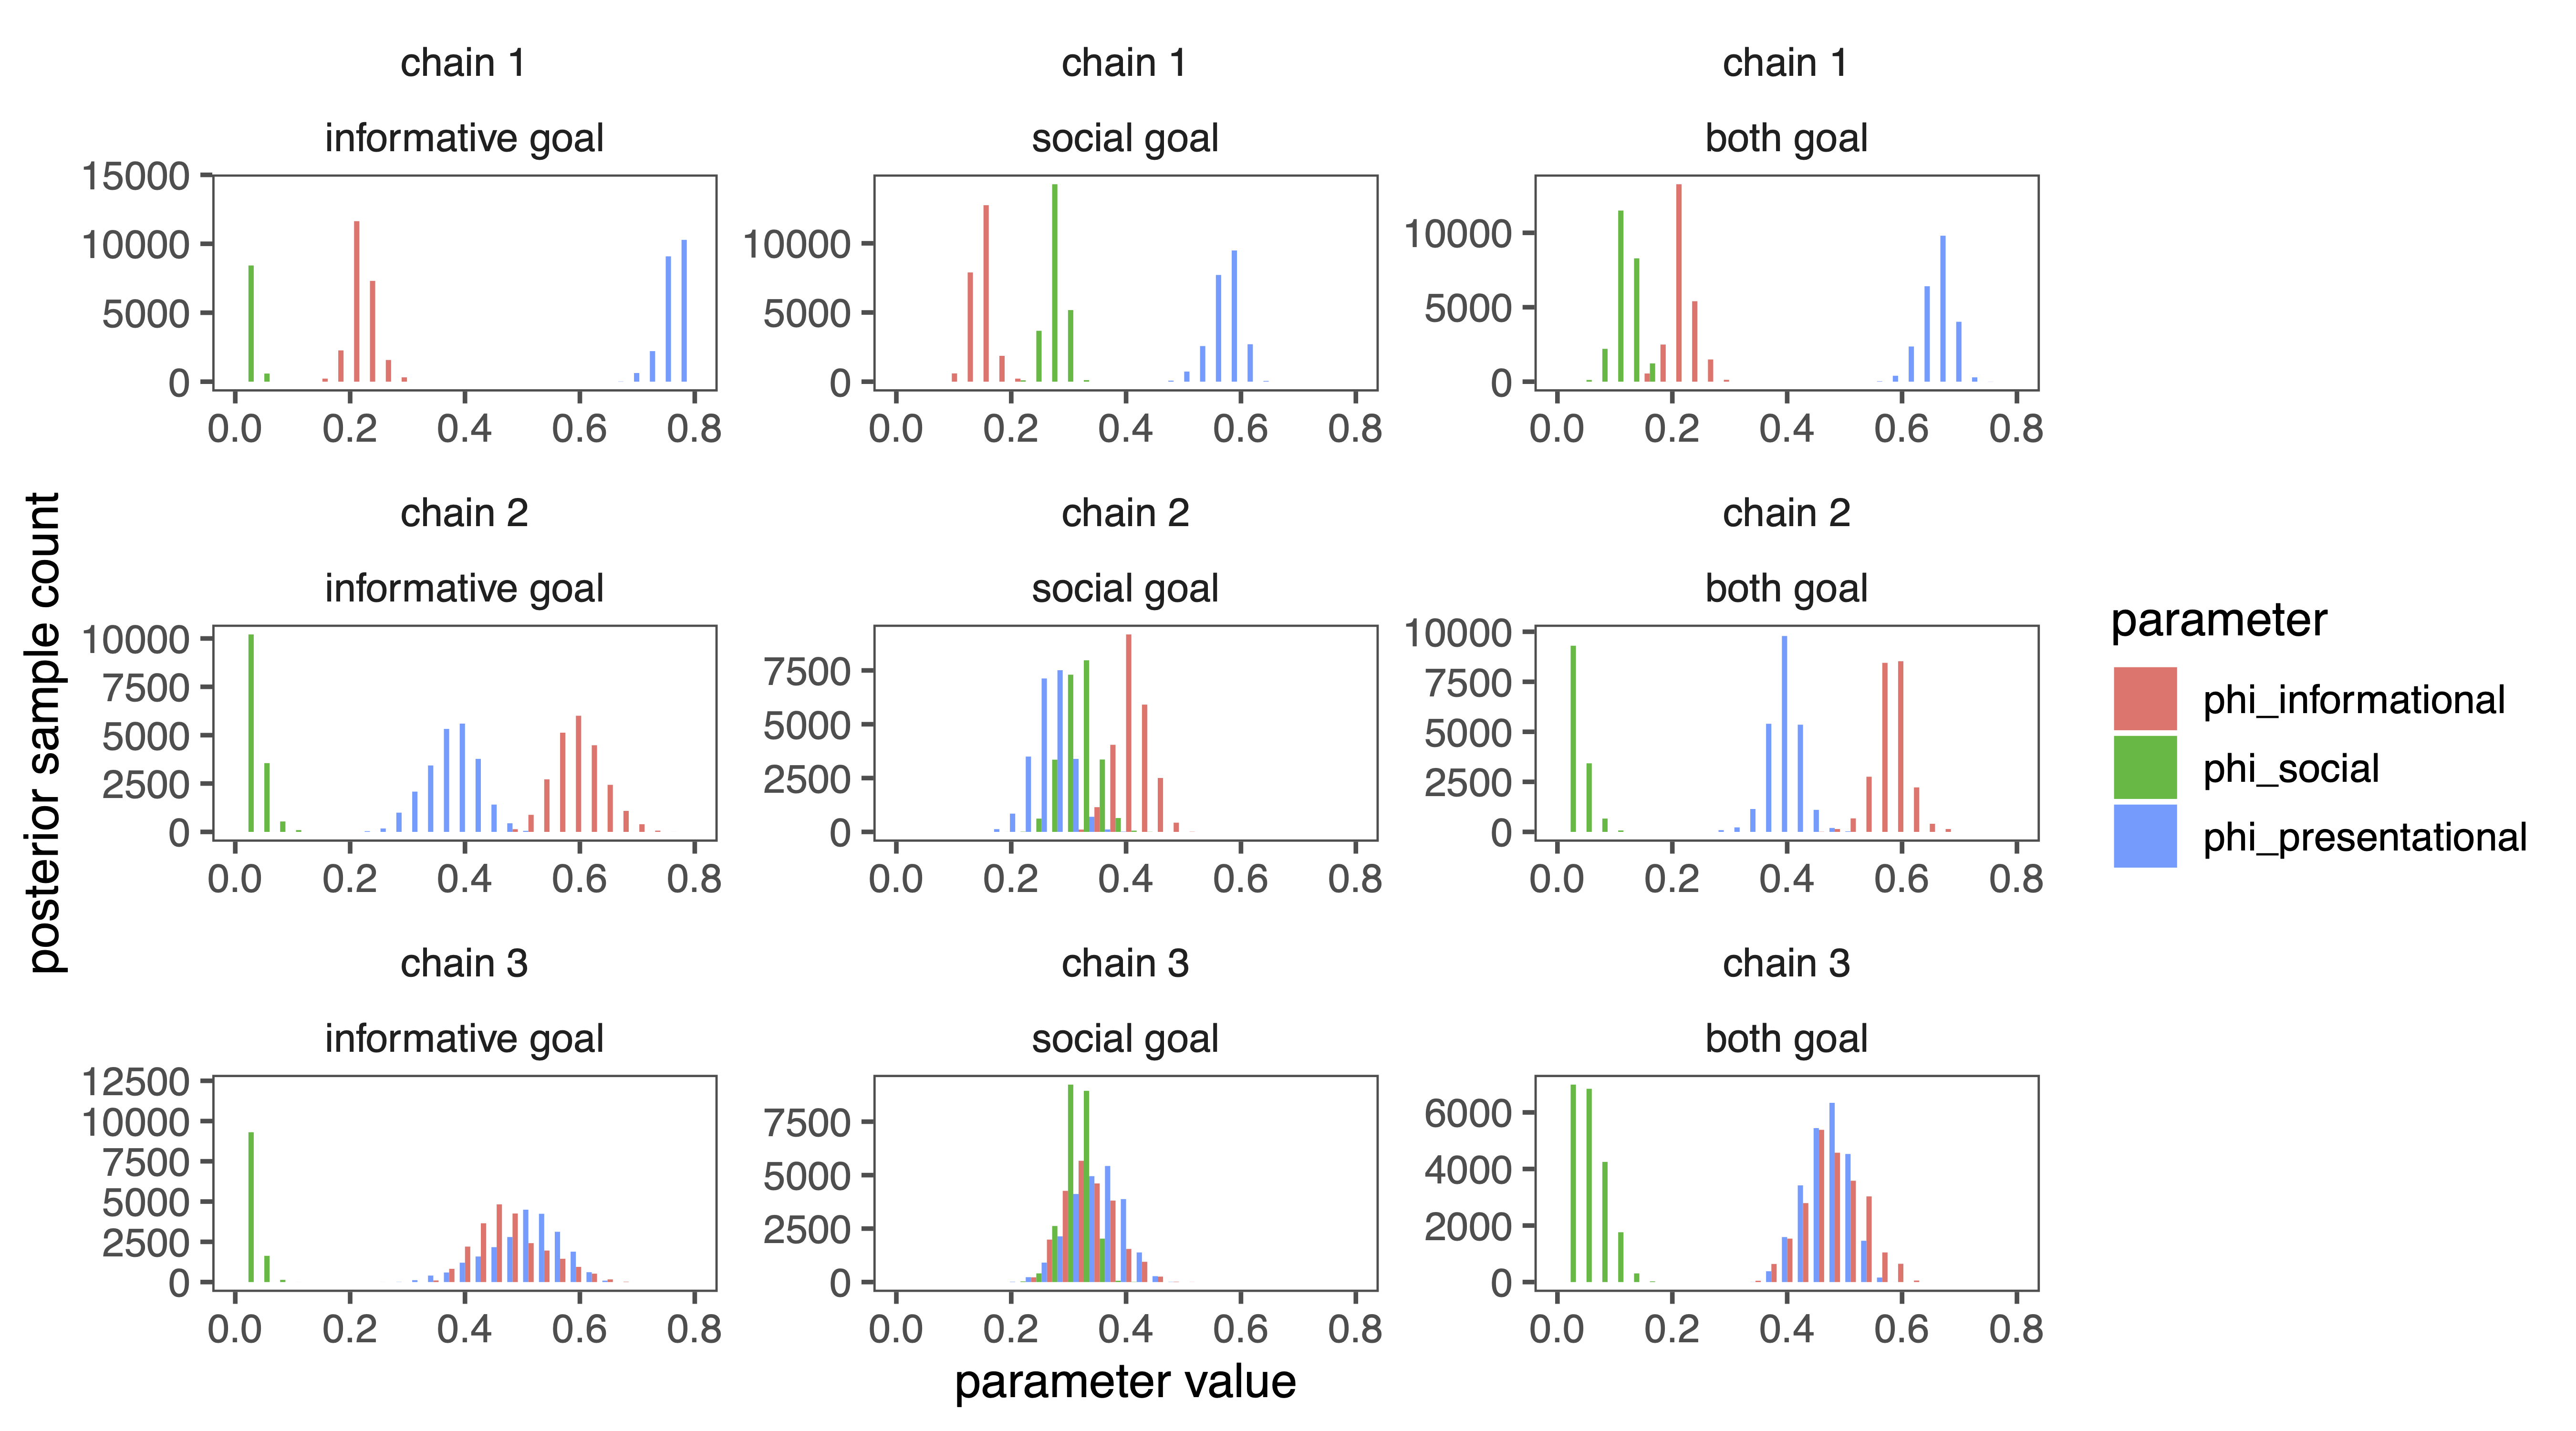
\includegraphics[width=0.7\linewidth]{fig/4chains_350k_phiKernel3_params_weights} 

}

\caption{A goal-centric view of the utility-weight parameters. Columns denote different goal conditions and rows denote different MCMC chains. There are substantial inconsistencies in the posterior distributions over utility-weights. Social utility appears most consistent.}\label{fig:posteriorParamByGoal}
\end{figure}

\begin{figure}[!h]

{\centering 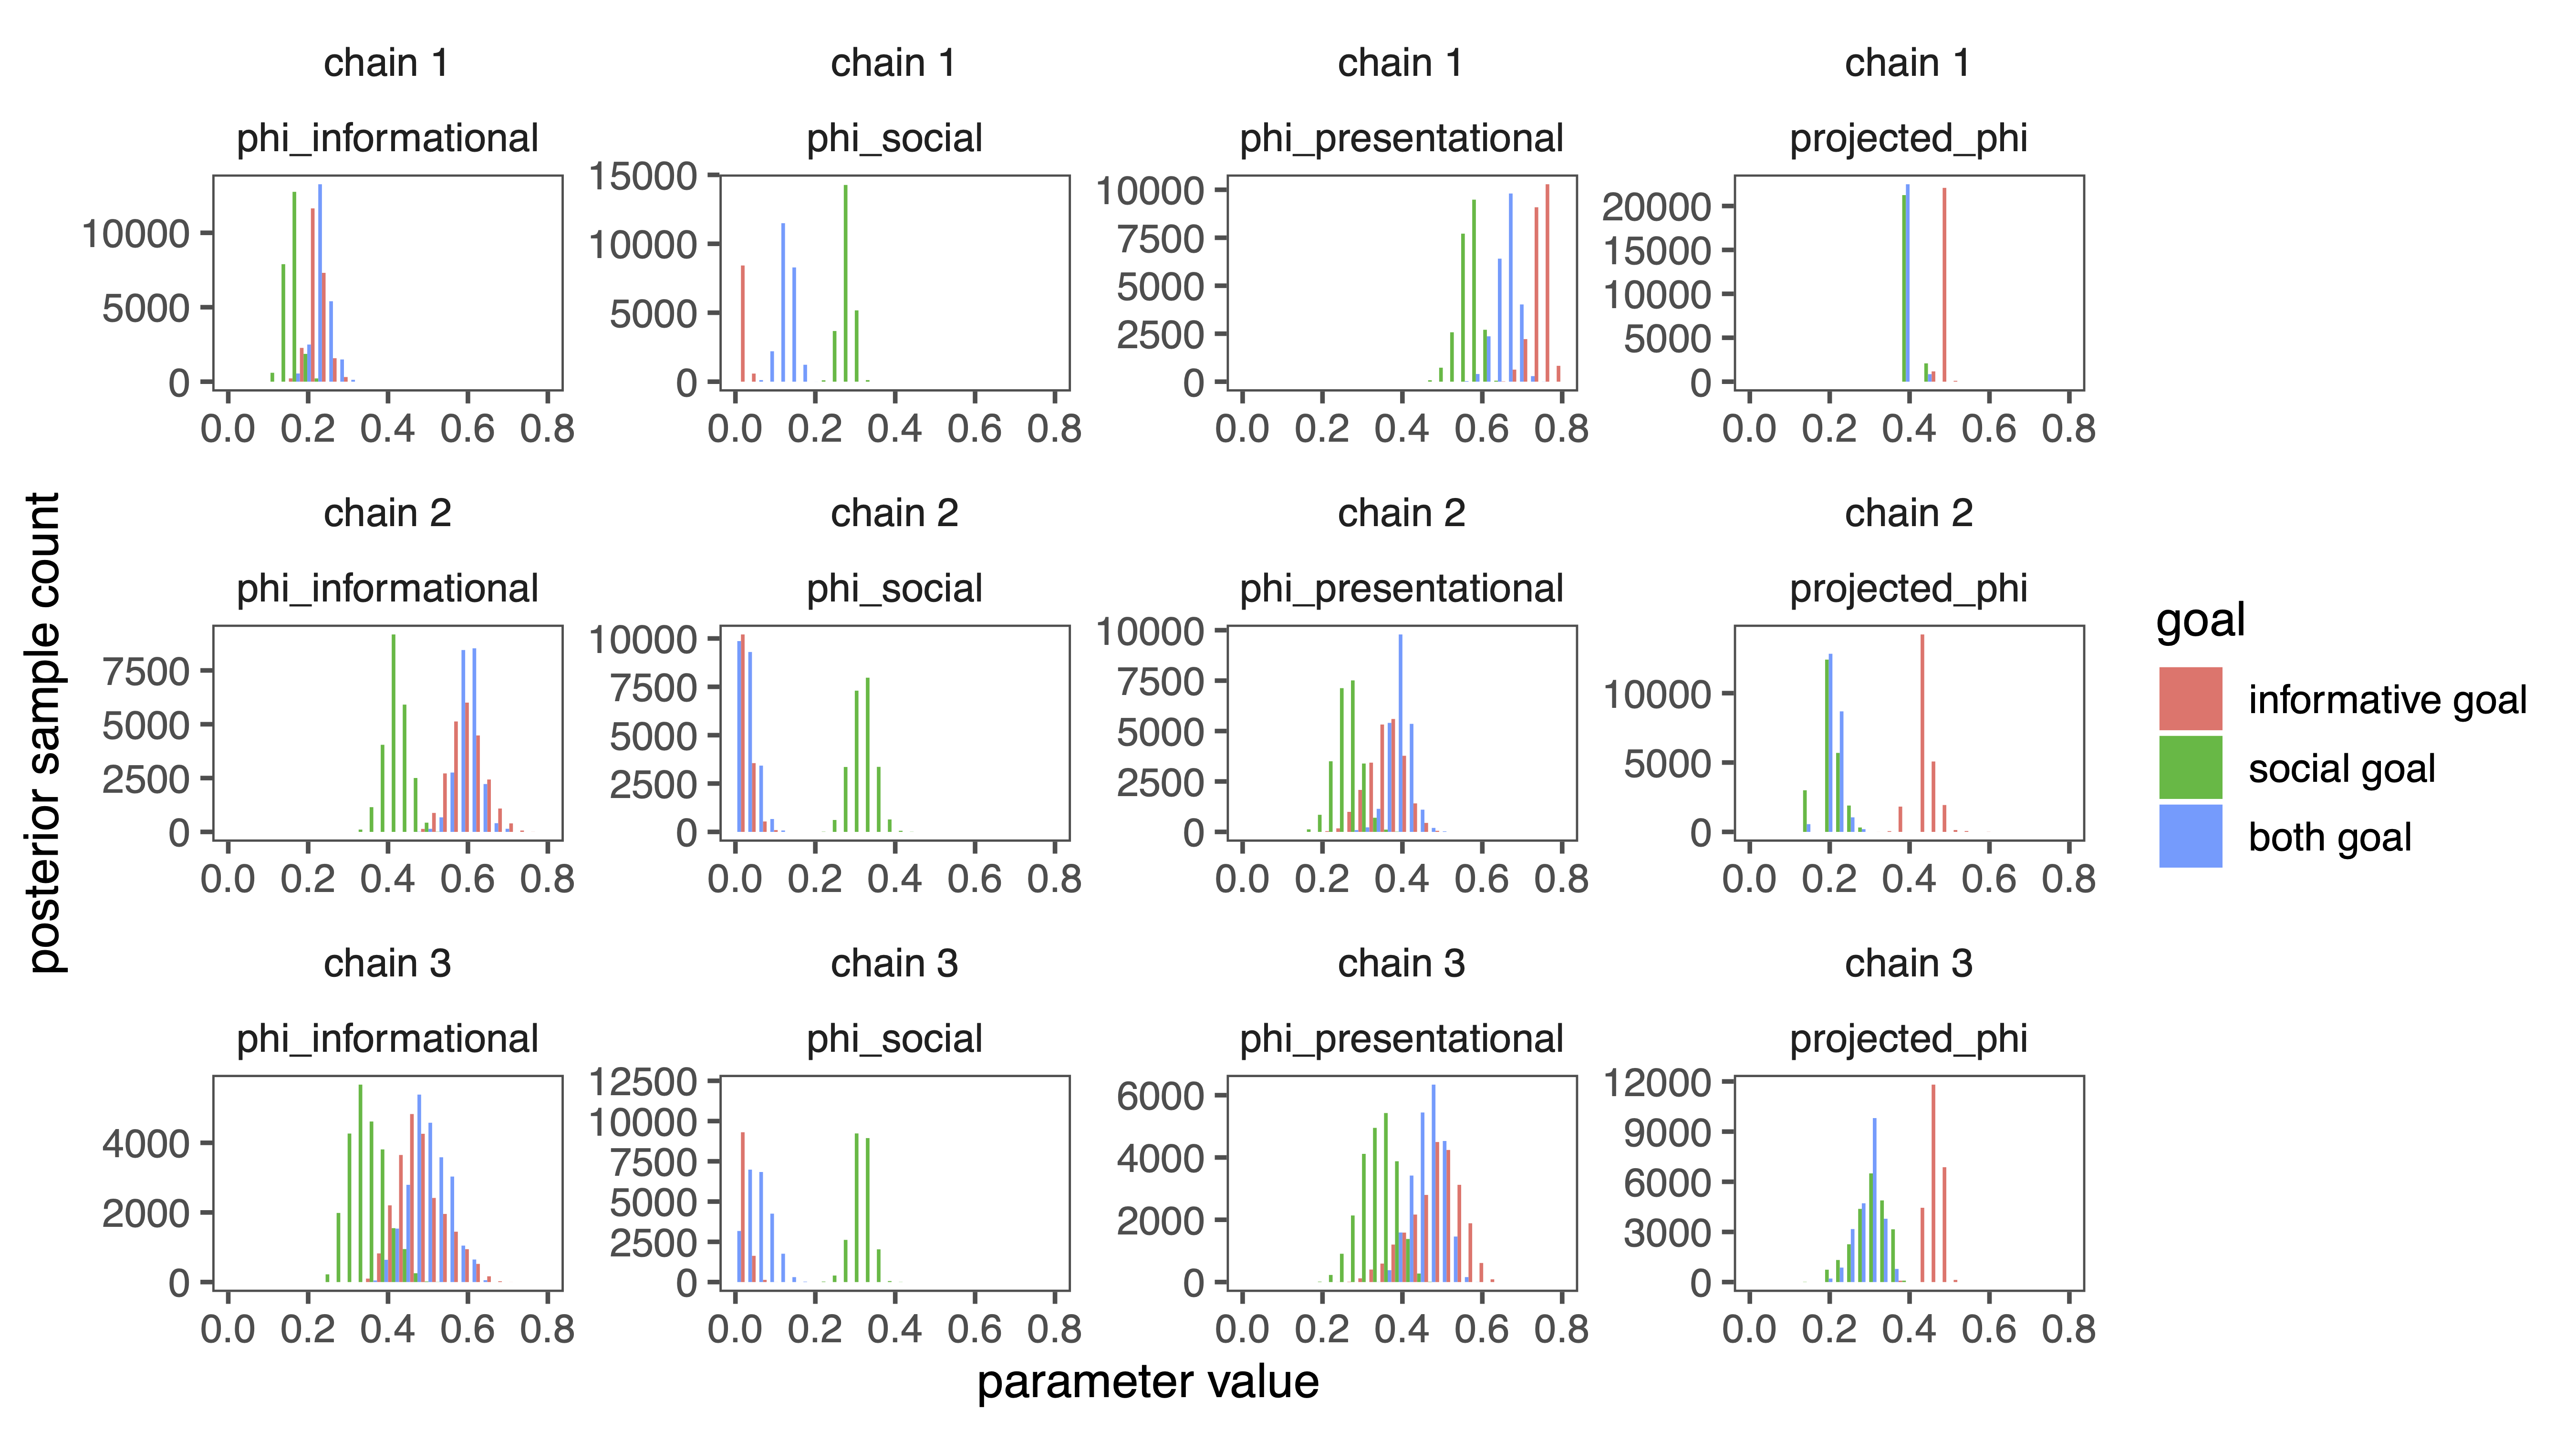
\includegraphics[width=0.7\linewidth]{fig/4chains_350k_phiKernel3_params_weights_v2} 

}

\caption{A utility-centric view of the utility-weight parameters. Relative orderings of the utility-weights across the different goal conditions are consistent.}\label{fig:posteriorParamByUtility}
\end{figure}

\newpage

\subsection{Data Availability}\label{data-availability}

Our model, preregistration of hypotheses, procedure, data, and analyses
are available at \url{https://github.com/ejyoon/polite_speaker}.

\newpage


\subsection{Supplemental Figures}\label{supplemental-figures}

\begin{figure}[!h]
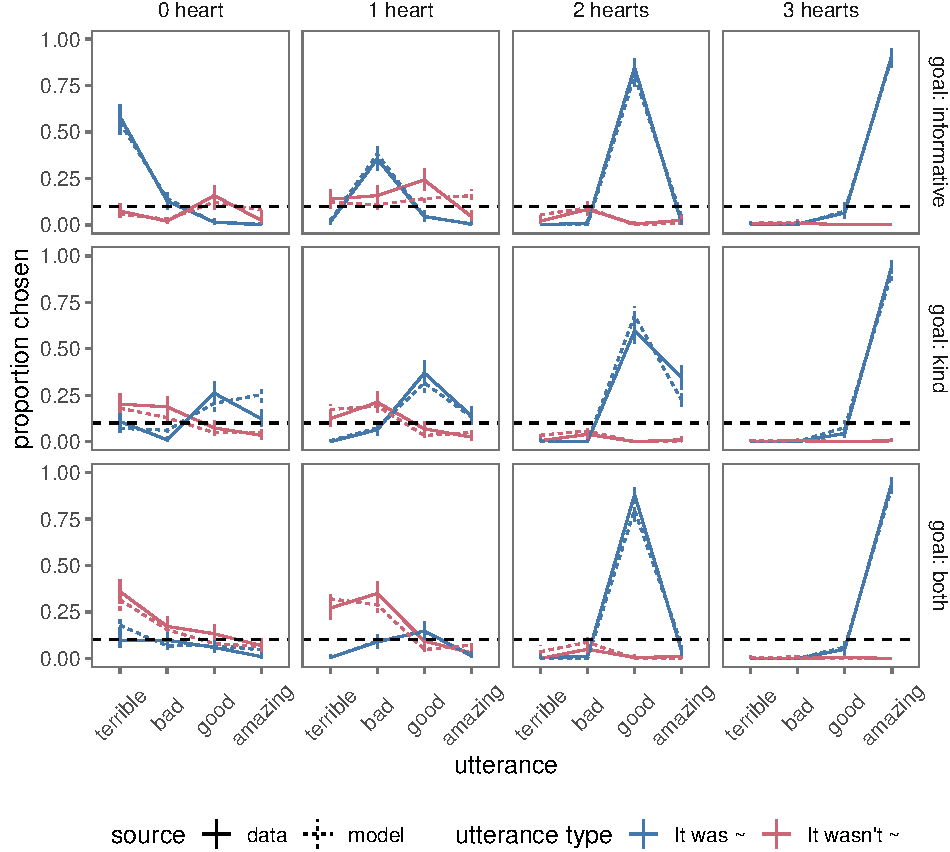
\includegraphics[width=\textwidth]{polite_manuscript_files/figure-latex/utterance-1} \caption{Experimental results (solid lines) and fitted predictions from the full model (dashed lines) for speaker production. Proportion of utterances chosen (utterance type – direct vs. indirect – in different colors and words shown on x-axis) given the true states (columns) and speaker goals (rows). Error bars represent 95\% confidence intervals for the data and 95\% highest density intervals for the model. Black dotted line represents the chance level.}\label{fig:utterance}
\end{figure}

\begin{figure}[!h]
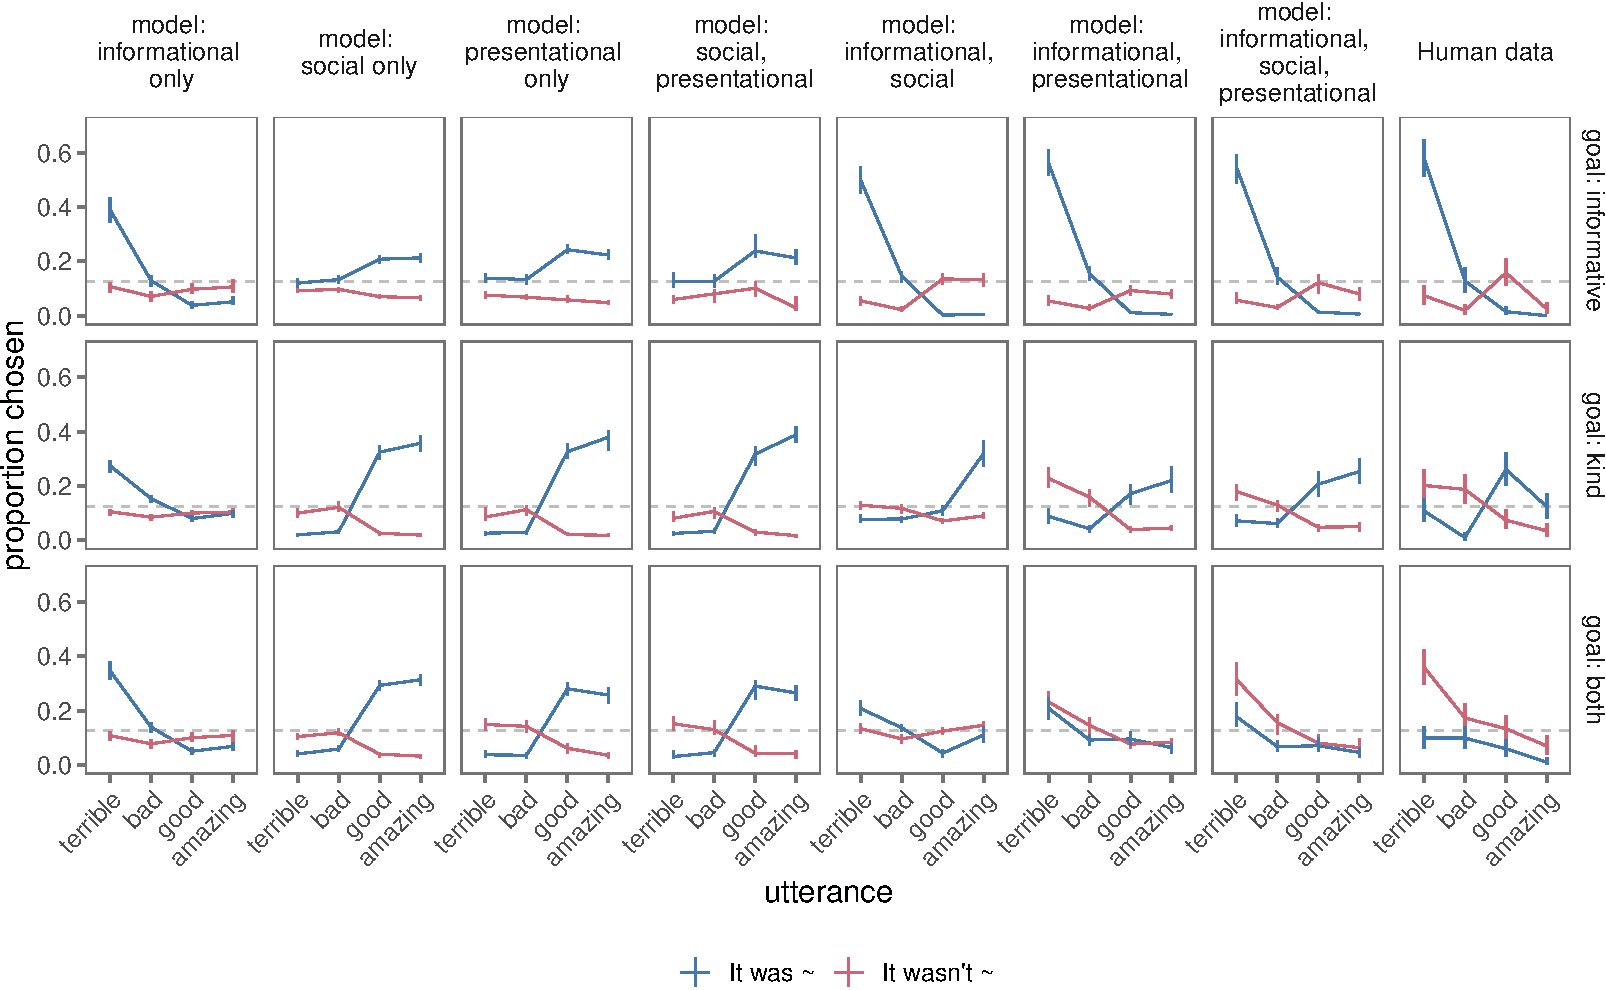
\includegraphics[width=\textwidth]{polite_manuscript_files/figure-latex/comparisonAll-1} \caption{Comparison of predictions for proportion of utterances chosen by pragmatic speaker from possible model variants (left) and human data (rightmost) for average proportion of negation produced among all utterances, given true state of 0 heart and speaker with a goal to be informative (top), kind (middle), or both (bottom). Gray dotted line indicates chance level at 12.5\%. Error bars represent 95\% confidence intervals for the data (rightmost) and 95\% highest density intervals for the models (left).}\label{fig:comparisonAll}
\end{figure}

\begin{figure}[!h]
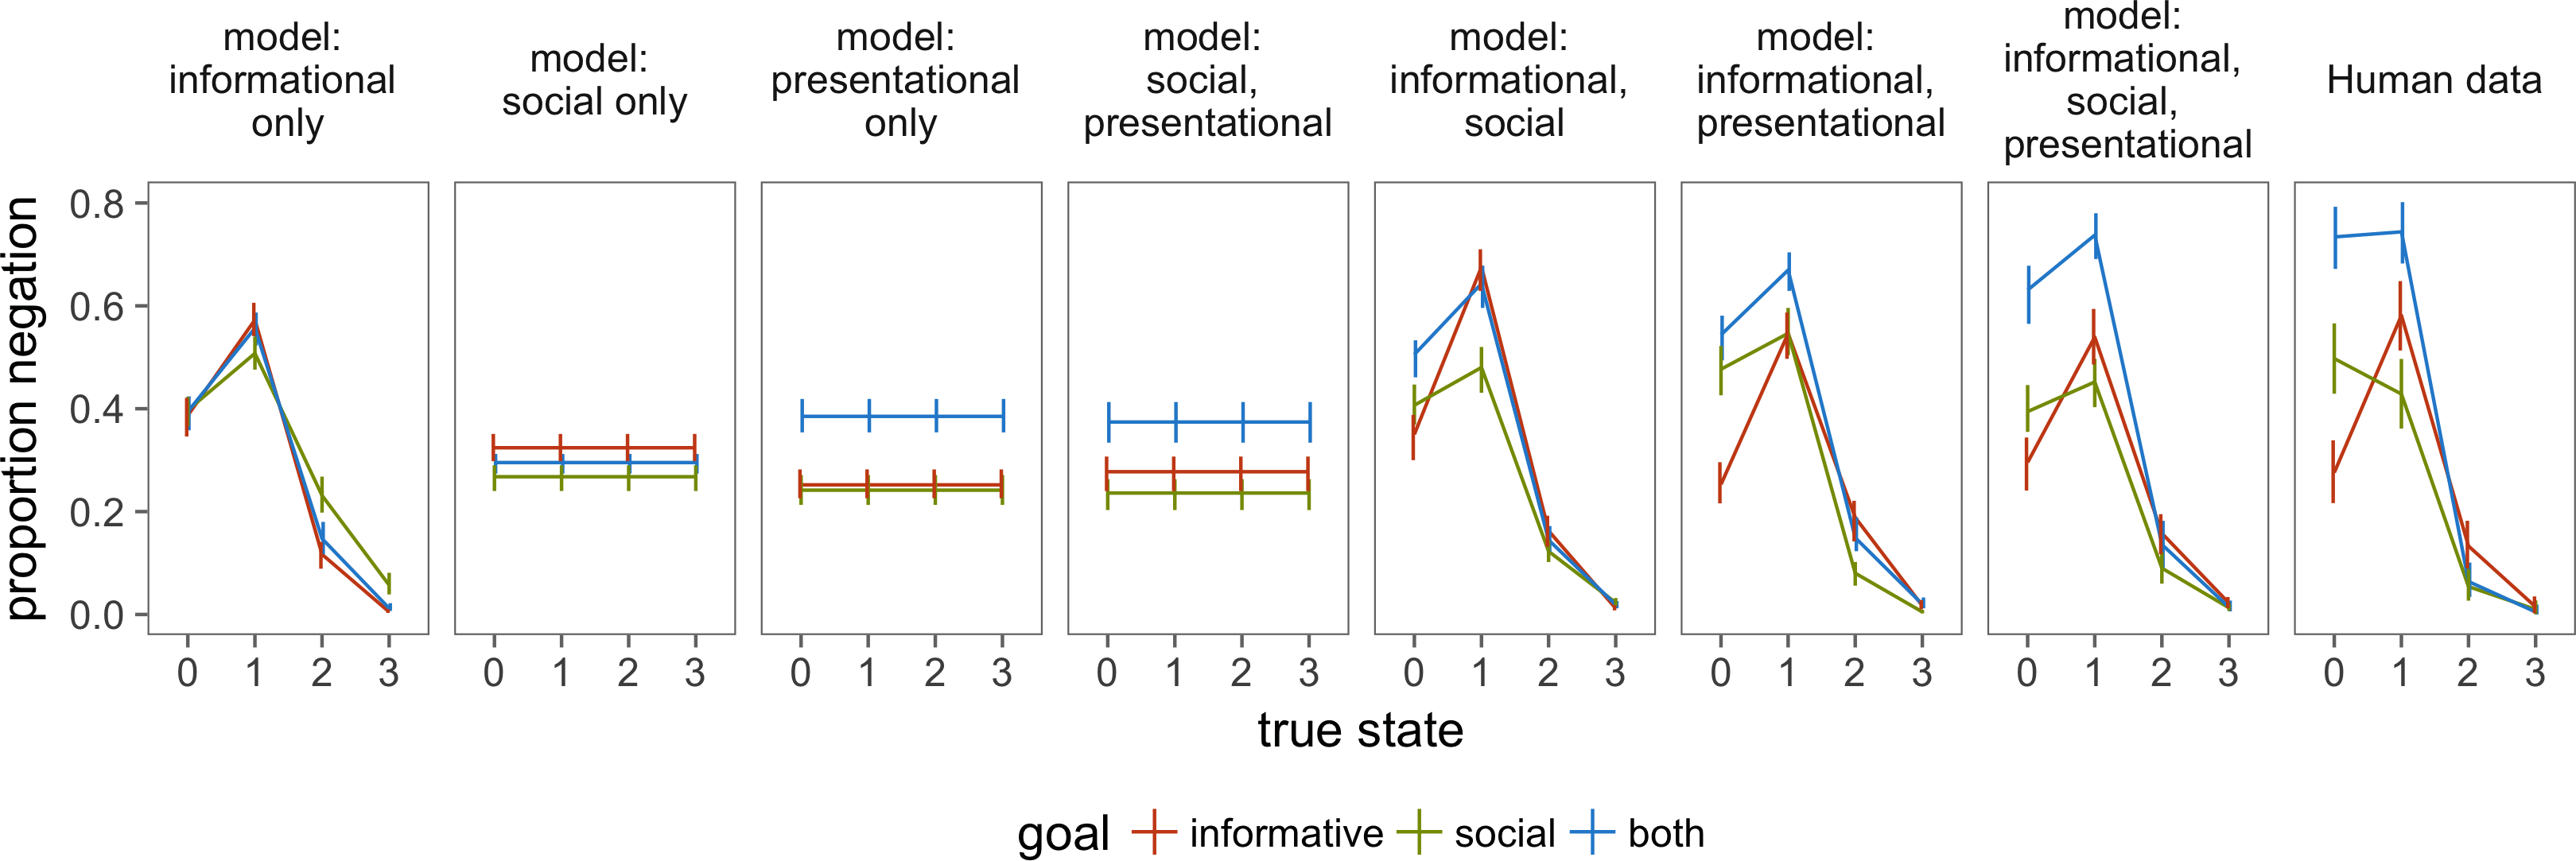
\includegraphics[width=\textwidth]{polite_manuscript_files/figure-latex/negation-1} \caption{Experimental results (left) and fitted model predictions (right) for average proportion of negation produced among all utterances, given true states (x-axis) and goals (colors).}\label{fig:negation}
\end{figure}

\newpage



%%% End of Article
%%% These elements should be used, with the exception of Appendices which
%%% are optional.

%%% \section{Supportive Information}
% \acknowledgments
% \authorcontributions 
% \bibliography{<name of .bib file>}
% \appendix % optional

%\section{Supportive Information}
%Here you enter further sources of information, if desired.

%% A possible entry might be:
% No supportive information is available at this time.

\acknowledgments
This work was supported by NSERC PGS Doctoral scholarship
    PGSD3-454094-2014 to EJY, NSF Graduate Research Fellowship DGE-114747 to
    MHT, ONR grant N00014-13-1-0788 and an Alfred P. Sloan Research
    Fellowship to NDG, and NSF grant BCS 1456077 to MCF.


%% ie.,

% The authors thank Laurence Aitchison for fruitful discussions.  RKN
% and PD received funding from the Gatsby Charitable Foundation. Y-AB,
% RBS, KC and PS received funding from Canadian Institutes of Health
% Research grant $MOP74577$,
% Fond de recherche Qu\'{e}bec - Sant\'{e} (Group grant to the Groupe 
% de recherche en neurobiologie comportementale, Shimon Amir, P.I.), and
% Concordia University Research Chair (Tier I). 

\authorcontributions 
 All authors designed research and wrote the paper; E.J.Y. and M.H.T.
    performed research and analyzed data. 

%% ie.
%% Project was formulated by RKN, PD, PS,
%% based on substantial data, analyses and experiments of Y-AB, KC, RS,
%% PS. RKN, PD formalised the model, RKN implemented and ran the model;
%% RKN analysed the molecular ethogram data; Y-AB formalised and
%% implemented a CTMC model. All authors wrote the manuscript.


%%%%%%%%%%%%%%%%%%%%%%%
%% The bibliography

%% The bibliography is made using only the entries that you cite using 
%% \cite{}, or one of the Natbib citation entries, like \citep{}, \citet{} etc.

\bibliography{politeness}

%ie.,
%\bibliography{bibsamp}

%% Optional Appendix
%\appendix

%\section{Sample Appendix Section}


\end{document}

\subsection{Sample Subsection}
Text here. Text here. Text here. Text here.
Text here. Text here. Text here. Text here.
Text here. Text here. Text here. Text here.
Text here. Text here. Text here. Text here.

\subsubsection{Sample Subsubsection}
Text here. Text here. Text here. Text here.
Text here. Text here. Text here. Text here.
Text here. Text here. Text here. Text here.
Text here. Text here. Text here. Text here.


\subsection{Simple code sample}

\begin{code}
\begin{verbatim}
procedure bubbleSort( A : list of sortable items )
    n = length(A)
    repeat
       newn = 0
       for i = 1 to n-1 inclusive do
          if A[i-1] > A[i] then
             swap(A[i-1], A[i])
             newn = i
          end if
       end for
       n = newn
    until n = 0
end procedure
\end{verbatim}
\end{code}



\subsection{Algorithm environment}

%% \begin{algorithm} takes option [p][b][t][h],  or some combination, like \begin{figure}
%% See documentation for algorithmic.sty for more information on formatting algorithms.

\begin{algorithm}[h]
\caption{A sample in an algorithm environment.}
\begin{algorithmic}
\If {$i\geq maxval$}
    \State $i\gets 0$
\Else
    \If {$i+k\leq maxval$}
        \State $i\gets i+k$
    \EndIf
\EndIf
\end{algorithmic}
\end{algorithm}


\section{Jargon definitions}

\begin{wideboxedtext}
\begin{glossary}
\symbol{Term} Definition
\symbol{Term} Definition
%ie
%\symbol{$1/\lambda$} mean of exponential effective prior probability density for leisure time
%\symbol{CHT} Cumulative Handling Time 
\end{glossary}
\end{wideboxedtext}

\begin{boxedtext}
\begin{glossary}
\symbol{Term} Definition
\symbol{Term} Definition
%ie
%\symbol{$1/\lambda$} mean of exponential effective prior probability density for leisure time
%\symbol{CHT} Cumulative Handling Time 
\end{glossary}
\end{boxedtext}

\section{Itemized Lists}

\subsection{Roman list:}

\begin{enumerate}
\item[(i)] at high 
payoffs, subjects work almost continuously, engaging in little leisure
in between work bouts; 
\item[(ii)] at low payoffs, they 
engage in leisure all at once, in long bouts after working, rather
than distributing the same amount of leisure time into multiple short
leisure bouts; 
\item[(iii)] subjects work continuously for the entire price duration, as long as
the price is not very long (as shown by an analysis conducted by Y-AB, to be published separately); %(\textbf{Figure \ref{fig:task_data}D}).
\item[(iv)] the duration of leisure bouts is variable.
\end{enumerate}

\subsection{Numbered list:}

\begin{enumerate}
\item at high 
payoffs, subjects work almost continuously, engaging in little leisure
inbetween work bouts; 
\item at low payoffs, they 
engage in leisure all at once, in long bouts after working, rather
than distributing the same amount of leisure time into multiple short
leisure bouts; 
\item subjects work continuously for the entire price duration, as long as
the price is not very long (as shown by an analysis conducted by Y-AB, to be published separately); %(\textbf{Figure \ref{fig:task_data}D}).
\item the duration of leisure bouts is variable.
\end{enumerate}


\subsection{Bulleted list:}

\begin{itemize}
\item at high 
payoffs, subjects work almost continuously, engaging in little leisure
inbetween work bouts; 
\item at low payoffs, they 
engage in leisure all at once, in long bouts after working, rather
than distributing the same amount of leisure time into multiple short
leisure bouts; 
\item subjects work continuously for the entire price duration, as long as
the price is not very long (as shown by an analysis conducted by Y-AB, to be published separately); %(\textbf{Figure \ref{fig:task_data}D}).
\item the duration of leisure bouts is variable.
\end{itemize}


\section{Sample citations}
For general information on the correct form for citations using
the APA 6 format, see the following sites:
\href{https://owl.english.purdue.edu/owl/resource/560/02/}
{APA 6, In-text citations, The Basics} and
\href{https://owl.english.purdue.edu/owl/resource/560/03/}
{APA 6, In-text citations}

\section{Natbib citation mark up}

\subsection{Single citations}
\noindent
\begin{tabular}{ll}
\bf Type&\bf Results\\
\hline
\verb+\citet{jon90}+&Jones et al. (1990)\\
\verb+\citet[chap. 2]{jon90}+&Jones et al. (1990, chap. 2)\\
    \verb+\citep{jon90}+	    &   	(Jones et al., 1990)\\
    \verb+\citep[chap. 2]{jon90}+ 	&    	(Jones et al., 1990, chap. 2)\\
    \verb+\citep[see][]{jon90}+ 	 &    	(see Jones et al., 1990)\\
    \verb+\citep[see][chap. 2]{jon90}+ 	&    	(see Jones et al., 1990, chap. 2)\\
    \verb+\citet*{jon90}+ 	    &    	Jones, Baker, and Williams (1990)\\
    \verb+\citep*{jon90}+	    &    	(Jones, Baker, and Williams,
    1990) \\
\end{tabular}

For example, some citations from the OpenMindSample bibliography:
citet:\citet{anderson}, citep:\citep{antibayes}, and
cite*: \citet*{anderson}.

\subsection{Multiple citations}
Multiple citations may be made by including more than one citation
key in the \verb+\cite+ command argument.

\noindent
\begin{tabular}{ll}
\bf Type&\bf Results\\
\hline
\verb+\citet{jon90,jam91}+&Jones et al. (1990); James et al. (1991)\\
\verb+\citep{jon90,jam91}+&(Jones et al., 1990; James et al. 1991)\\
\verb+\citep{jon90,jon91}+&(Jones et al., 1990, 1991)\\
\verb+\citep{jon90a,jon90b}+&(Jones et al., 1990a,b)\\
\end{tabular}

For example, multiple citations from the OpenMindSample bibliography:
citet:\citet{anderson,antibayes}, citep:\citep{anderson,antibayes}.
As you see, the citations are automatically hyperlinked to their
reference in the bibliography.

\newpage

\section{Sample figures}

\begin{figure}[h] 
\centerline{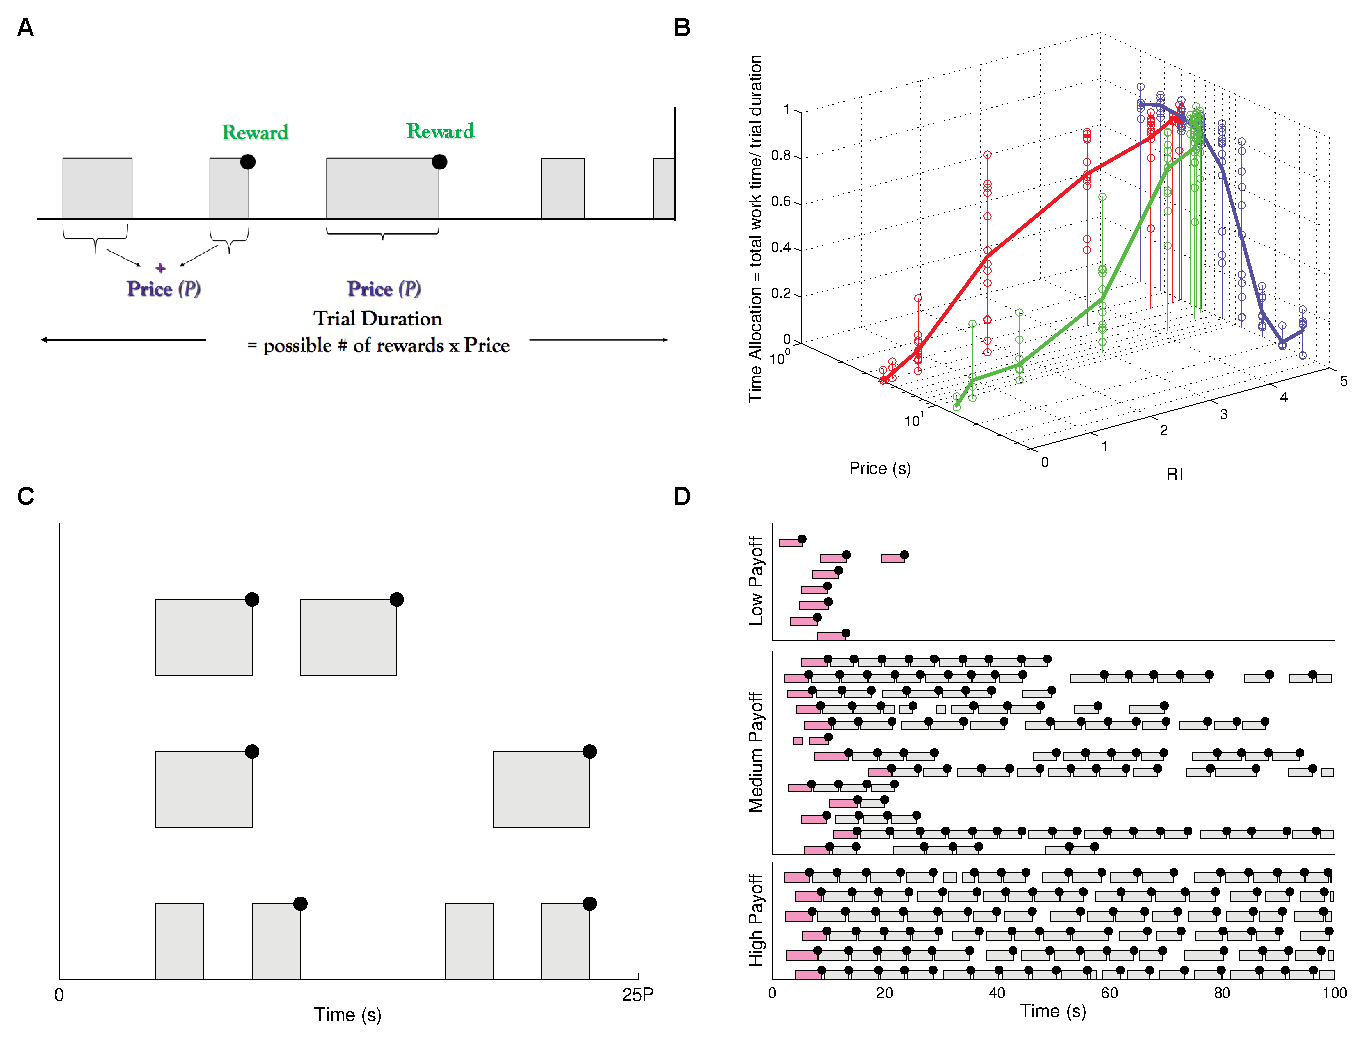
\includegraphics[width=\textwidth]{Fig1}}
\caption{(Colour online) \textbf{Task and key features of the
 data.} \\
 A) Cumulative handling time (CHT) task. Grey bars denote work
(depressing a lever), white gaps show leisure. The subject must
 accumulate work up to a total period of time called the
\emph{price} ($P$) in order to obtain a single reward (black dot) of subjective reward
intensity $RI$. The trial duration is $25\times \mathrm{price}$ (plus
$2$s each time the price is attained, during which the lever is retracted so it cannot
work; not shown).
}
\label{fig:task_data}
\end{figure}

\begin{figure}[ht] 
\widefigure{\fullpagewidth}{Fig1}
\caption{(Colour online) \textbf{Task and key features of the
 data.} \\
A) Cumulative handling time (CHT) task. Grey bars denote work
(depressing a lever), white gaps show leisure. The subject must
accumulate work up to a total period of time called the
\emph{price} ($P$) in order to obtain a single reward (black dot) of subjective reward
intensity $RI$. The trial duration is $25\times \mathrm{price}$ (plus
$2$s each time the price is attained, during which the lever is retracted so it cannot
work; not shown).
}
\label{newfig:task_data}
\end{figure}

\clearpage
\section{Sample tables}

\begin{table}[!ht]
\caption{Time of the Transition Between Phase 1 and Phase 2$^{a}$}
\label{tab:label}
\centering
\begin{tabular}{lc}
\hline
 Run  & Time (min)  \\
\hline
  $l1$  & 260   \\
  $l2$  & 300   \\
  $l3$  & 340   \\
  $h1$  & 270   \\
  $h2$  & 250   \\
  $h3$  & 380   \\
  $r1$  & 370   \\
  $r2$  & 390   \\
\hline
\multicolumn{2}{l}{$^{a}$Table note text here.}
\end{tabular}
\end{table}

\begin{table}[ht]
\widecaption{Sample table taken from [treu03]\label{tbl-1}}
\begin{widetable}
\advance\tabcolsep-1pt
\small
\begin{tabular}{ccrrccccccccc}
\hline
\bf 
POS &\bf  chip &\multicolumn1c{\bf ID} &\multicolumn1c{\bf X}
&\multicolumn1c{\bf Y} &\bf
RA &\bf DEC &\bf IAU$\pm$ $\delta$ IAU &\bf
IAP1$\pm$ $\delta$ IAP1 &\bf IAP2 $\pm$ $\delta$
IAP2 &\bf star &\bf E &\bf Comment\\
\hline
0 & 2 & 1 & 1370.99 & 57.35\rlap{$^a$}    &   6.651120 &  17.131149 &
21.344$\pm$0.006\rlap{$^b$}  & 2 4.385$\pm$0.016 & 23.528$\pm$0.013 & 0.0 & 9 & -    \\
0 & 2 & 2 & 1476.62 & 8.03     &   6.651480 &  17.129572 & 21.641$\pm$0.005  & 2 3.141$\pm$0.007 & 22.007$\pm$0.004 & 0.0 & 9 & -    \\
0 & 2 & 3 & 1079.62 & 28.92    &   6.652430 &  17.135000 & 23.953$\pm$0.030  & 2 4.890$\pm$0.023 & 24.240$\pm$0.023 & 0.0 & - & -    \\
0 & 2 & 4 & 114.58  & 21.22    &   6.655560 &  17.148020 & 23.801$\pm$0.025  & 2 5.039$\pm$0.026 & 24.112$\pm$0.021 & 0.0 & - & -    \\
0 & 2 & 5 & 46.78   & 19.46    &   6.655800 &  17.148932 & 23.012$\pm$0.012  & 2 3.924$\pm$0.012 & 23.282$\pm$0.011 & 0.0 & - & -    \\
0 & 2 & 6 & 1441.84 & 16.16    &   6.651480 &  17.130072 & 24.393$\pm$0.045  & 2 6.099$\pm$0.062 & 25.119$\pm$0.049 & 0.0 & - & -    \\
0 & 2 & 7 & 205.43  & 3.96     &   6.655520 &  17.146742 & 24.424$\pm$0.032  & 2 5.028$\pm$0.025 & 24.597$\pm$0.027 & 0.0 & - & -    \\
0 & 2 & 8 & 1321.63 & 9.76     &   6.651950 &  17.131672 &
22.189$\pm$0.011  & 2 4.743$\pm$0.021 & 23.298$\pm$0.011 & 0.0 & 4 &
edge \\
\hline
\multicolumn{13}{l}{%
Table 2 is published in its entirety in the electronic
edition of the {\it Astrophysical Journal}.}\\[3pt]
\multicolumn{13}{l}{%
$^a$ Sample footnote for table 2.}\\[3pt]
\multicolumn{13}{l}{%
$^b$ Another sample footnote for table 2.}
\end{tabular}
\end{widetable}
\end{table}

\begin{table}[p]
\rotatebox{90}{\vbox{\hsize=\textheight
\caption{Here is a caption for a table that is found in landscape
mode.}
\begin{tabular}{ccrrccccccccc}
\hline
\bf 
POS &\bf  chip &\multicolumn1c{\bf ID} &\multicolumn1c{\bf X}
&\multicolumn1c{\bf Y} &\bf
RA &\bf DEC &\bf IAU$\pm$ $\delta$ IAU &\bf
IAP1$\pm$ $\delta$ IAP1 &\bf IAP2 $\pm$ $\delta$
IAP2 &\bf star &\bf E &\bf Comment\\
\hline
0 & 2 & 1 & 1370.99 & 57.35\rlap{$^a$}    &   6.651120 &  17.131149 &
21.344$\pm$0.006\rlap{$^b$}  & 2 4.385$\pm$0.016 & 23.528$\pm$0.013 & 0.0 & 9 & -    \\
0 & 2 & 2 & 1476.62 & 8.03     &   6.651480 &  17.129572 & 21.641$\pm$0.005  & 2 3.141$\pm$0.007 & 22.007$\pm$0.004 & 0.0 & 9 & -    \\
0 & 2 & 3 & 1079.62 & 28.92    &   6.652430 &  17.135000 & 23.953$\pm$0.030  & 2 4.890$\pm$0.023 & 24.240$\pm$0.023 & 0.0 & - & -    \\
0 & 2 & 4 & 114.58  & 21.22    &   6.655560 &  17.148020 & 23.801$\pm$0.025  & 2 5.039$\pm$0.026 & 24.112$\pm$0.021 & 0.0 & - & -    \\
0 & 2 & 5 & 46.78   & 19.46    &   6.655800 &  17.148932 & 23.012$\pm$0.012  & 2 3.924$\pm$0.012 & 23.282$\pm$0.011 & 0.0 & - & -    \\
0 & 2 & 6 & 1441.84 & 16.16    &   6.651480 &  17.130072 & 24.393$\pm$0.045  & 2 6.099$\pm$0.062 & 25.119$\pm$0.049 & 0.0 & - & -    \\
0 & 2 & 7 & 205.43  & 3.96     &   6.655520 &  17.146742 & 24.424$\pm$0.032  & 2 5.028$\pm$0.025 & 24.597$\pm$0.027 & 0.0 & - & -    \\
0 & 2 & 8 & 1321.63 & 9.76     &   6.651950 &  17.131672 &
22.189$\pm$0.011  & 2 4.743$\pm$0.021 & 23.298$\pm$0.011 & 0.0 & 4 &
edge \\
\hline
\multicolumn{13}{l}{%
Table 2 is published in its entirety in the electronic
edition of the {\it Astrophysical Journal}.}\\[3pt]
\multicolumn{13}{l}{%
$^a$ Sample footnote for table 2.}\\[3pt]
\multicolumn{13}{l}{%
$^b$ Another sample footnote for table 2.}
\end{tabular}
}}
\end{table}
\clearpage


\vglue 3in
Example of table continuing over pages:


\begin{center}
\begin{longtable}{ccc@{}}
\caption{ApJ costs from 1991 to 2013
\label{tab:table}} \\[2pt]
\hline
\bf Year & \bf Subscription & \bf Publication \\
 & \bf cost &\bf charges\\
 & \bf(\$) & \bf (\$/page)\\
\hline
\endfirsthead

\multicolumn3c{Table \thetable, \it continued from previous page.}\\[6pt]
\multicolumn3c{ApJ costs from 1991 to 2013}\\[2pt]
\hline
\bf Year & \bf Subscription & \bf Publication \\
 & \bf cost &\bf charges\\
 & \bf(\$) & \bf (\$/page)\\
\hline
\endhead
\\\hline
\\[-8pt]
\multicolumn{3}{r}{\it Table continued on next page}\\ 
\endfoot

\hline
\endlastfoot

1991 & 600 & 100 \\
1992 & 650 & 105 \\
1993 & 550 & 103 \\
1994 & 450 & 110 \\
1995 & 410 & 112 \\
1996 & 400 & 114 \\
1997 & 525 & 115 \\
1998 & 590 & 116 \\
1999 & 575 & 115 \\
2000 & 450 & 103 \\
2001 & 490 &  90 \\
2002 & 500 &  88 \\
2003 & 450 &  90 \\
2004 & 460 &  88 \\
2005 & 440 &  79 \\
2006 & 350 &  77 \\
2007 & 325 &  70 \\
2008 & 320 &  65 \\
2009 & 190 &  68 \\
2010 & 280 &  70 \\
2011 & 275 &  68 \\
2012 & 150 &  56 \\
2013 & 140 &  55 \\
\end{longtable}
\end{center}

\section{Supportive Information}
Here you enter further sources of information, if desired.

%% A possible entry might be:
% No supportive information is available at this time.


\acknowledgments
Enter your acknowledgments here.

%% ie.,

% The authors thank Laurence Aitchison for fruitful discussions.  RKN
% and PD received funding from the Gatsby Charitable Foundation. Y-AB,
% RBS, KC and PS received funding from Canadian Institutes of Health
% Research grant $MOP74577$,
% Fond de recherche Qu\'{e}bec - Sant\'{e} (Group grant to the Groupe 
% de recherche en neurobiologie comportementale, Shimon Amir, P.I.), and
% Concordia University Research Chair (Tier I). 

\authorcontributions 
Who helped formulate the project, who supplied data, analyses and
experiments, etc.

%% ie.
%% Project was formulated by RKN, PD, PS,
%% based on substantial data, analyses and experiments of Y-AB, KC, RS,
%% PS. RKN, PD formalised the model, RKN implemented and ran the model;
%% RKN analysed the molecular ethogram data; Y-AB formalised and
%% implemented a CTMC model. All authors wrote the manuscript.


%%%%%%%%%%%%%%%%%%%%%%%
%% The bibliography

%% \nocite{*} is used here as a quick way to get every entry  in the .bib file to
%% appear in the bibliography. Normally the bibliography is made using only
%% the bibentries that you cite using \cite{}, or one of the Natbib citation
%% entries, like \citep{}, \citet{} etc.

\nocite{*}
\bibliography{bibsamp}


\appendix

\section{Sample Appendix Section}
We derive the result in Eq. \eqref{eq:analytical_linear}. We consider a linear $C_L(\tau_L+\taupav)=K_L(\tau_L+\taupav)$, and
make two further 
simplifications: (i) the subject does not
engage in leisure in the pre-reward state (and so works for the whole
price when it works); and (ii) \emph{a priori}, arbitrarily long leisure durations are possible
($\lambda=0$).
Then the reward rate in Eq. \eqref{eq:rhoCHT} becomes
\begin{equation}\label{eq:analyticalrho}
\rho^{\pi}= \frac{\vrule height 10pt width0pt RI + K_L \{~ \mathbb{E}[ \tau_L | \textrm{post} ] + \taupav  \} }
     {P +
\mathbb{E}[ \tau_L | \textrm{post} ] +\taupav  } 
\end{equation} 
As discussed in the \emph{Results} section, the probability of engaging in instrumental leisure in the post-reward state is $\pi([L,\tau_L]
~| \textrm{post}) = \exp\left[-\{\beta (\rho^\pi-K_L) 
 \} \tau_L\right]$, which is an exponential distribution with
mean 
\begin{equation}
\mathbb{E}[\tau_L | \textrm{post}]=\frac{1}{\beta (\rho^\pi-K_L) }
\label{eq:analyticaltauL}
\end{equation}  
Re-arranging terms of this equation,
\begin{equation}\label{eq:rhoversion2}
\rho^{\pi}=\frac{1}{\beta ~\mathbb{E}[\tau_L | \textrm{post}]} +K_L 
\end{equation} 
Equating Eqs. \eqref{eq:analyticalrho} and \eqref{eq:rhoversion2} and solving for the mean instrumental leisure duration $\mathbb{E}[\tau_L | \textrm{post}]$, we derive
\begin{equation}
\mathbb{E}[\tau_L | \textrm{post}] = \frac{P+\taupav}{\beta ( RI - K_LP)-1} 
\label{eq:solvedtauL}
\end{equation}
which is the second line of Eq.\eqref{eq:analytical_linear}. This is the mean instrumental leisure duration as long as  $RI - K_LP>1$, and  $\mathbb{E}[\tau_L | \textrm{post}] \rightarrow \infty$ otherwise. When the former condition holds, we may
substitute Eq. \eqref{eq:solvedtauL} into Eq. \eqref{eq:analyticalrho} and solve for $\rho^{\pi}$
\begin{figure}
\widefigure{\fullpagewidth}{Fig1}
\caption{Sample Appendix Caption}
\end{figure}

\newpage

\section{Making Your Bibliography for an Open Mind Article}
{\it Open Mind} uses the APA author-date  bibliography style,
apacite.bst. For more
information on apacite, for examples in how to make your .bib file and more, see:\\
\href{http://mirror.jmu.edu/pub/CTAN/biblio/bibtex/contrib/apacite/apacite.pdf}
{http://mirror.jmu.edu/pub/CTAN/biblio/bibtex/contrib/apacite/apacite.pdf}

\noindent
(In spite of the mention of apacite cite commands, please use only
Natbib commands for in text citations, as shown above.)

\subsection{BibTeX}
You will need to use BibTeX to form your bibliography; typing in the
references would be
a huge and unpleasant task. Look at the openmindsample.bbl file and you'll see why
typing in the bibitems would be difficult. 

For a good basic introduction to using BibTeX, see
\href{https://www.economics.utoronto.ca/osborne/latex/BIBTEX.HTM}
{https://www.economics.utoronto.ca/osborne/latex/BIBTEX.HTM}

When you use BibTeX, the form of the bibliography will be correct. You
don't need to supply a bibliography style, since that is built into
the stjour.cls file.

\end{document}

